\documentclass[fleqn,10pt]{latex/stylish_article} % Document font size and equations flushed left

\setcounter{tocdepth}{3} % sections, subsections and subsubsections

% Pandoc environments
\usepackage{framed}
\usepackage{fancyvrb}
\providecommand{\tightlist}{%
  \setlength{\itemsep}{0pt}\setlength{\parskip}{0pt}}
\newcommand{\VerbBar}{|}
\newcommand{\VERB}{\Verb[commandchars=\\\{\}]}
\DefineVerbatimEnvironment{Highlighting}{Verbatim}{commandchars=\\\{\}, fontsize=\scriptsize} % R Code

% Colored code
\usepackage{color}
\definecolor{shadecolor}{RGB}{248,248,248}
\newenvironment{Shaded}{\begin{snugshade}}{\end{snugshade}}
\newcommand{\KeywordTok}[1]{\textcolor[rgb]{0.13,0.29,0.53}{\textbf{{#1}}}}
\newcommand{\DataTypeTok}[1]{\textcolor[rgb]{0.13,0.29,0.53}{{#1}}}
\newcommand{\DecValTok}[1]{\textcolor[rgb]{0.00,0.00,0.81}{{#1}}}
\newcommand{\BaseNTok}[1]{\textcolor[rgb]{0.00,0.00,0.81}{{#1}}}
\newcommand{\FloatTok}[1]{\textcolor[rgb]{0.00,0.00,0.81}{{#1}}}
\newcommand{\ConstantTok}[1]{\textcolor[rgb]{0.00,0.00,0.00}{{#1}}}
\newcommand{\CharTok}[1]{\textcolor[rgb]{0.31,0.60,0.02}{{#1}}}
\newcommand{\SpecialCharTok}[1]{\textcolor[rgb]{0.00,0.00,0.00}{{#1}}}
\newcommand{\StringTok}[1]{\textcolor[rgb]{0.31,0.60,0.02}{{#1}}}
\newcommand{\VerbatimStringTok}[1]{\textcolor[rgb]{0.31,0.60,0.02}{{#1}}}
\newcommand{\SpecialStringTok}[1]{\textcolor[rgb]{0.31,0.60,0.02}{{#1}}}
\newcommand{\ImportTok}[1]{{#1}}
\newcommand{\CommentTok}[1]{\textcolor[rgb]{0.56,0.35,0.01}{\textit{{#1}}}}
\newcommand{\DocumentationTok}[1]{\textcolor[rgb]{0.56,0.35,0.01}{\textbf{\textit{{#1}}}}}
\newcommand{\AnnotationTok}[1]{\textcolor[rgb]{0.56,0.35,0.01}{\textbf{\textit{{#1}}}}}
\newcommand{\CommentVarTok}[1]{\textcolor[rgb]{0.56,0.35,0.01}{\textbf{\textit{{#1}}}}}
\newcommand{\OtherTok}[1]{\textcolor[rgb]{0.56,0.35,0.01}{{#1}}}
\newcommand{\FunctionTok}[1]{\textcolor[rgb]{0.00,0.00,0.00}{{#1}}}
\newcommand{\VariableTok}[1]{\textcolor[rgb]{0.00,0.00,0.00}{{#1}}}
\newcommand{\ControlFlowTok}[1]{\textcolor[rgb]{0.13,0.29,0.53}{\textbf{{#1}}}}
\newcommand{\OperatorTok}[1]{\textcolor[rgb]{0.81,0.36,0.00}{\textbf{{#1}}}}
\newcommand{\BuiltInTok}[1]{{#1}}
\newcommand{\ExtensionTok}[1]{{#1}}
\newcommand{\PreprocessorTok}[1]{\textcolor[rgb]{0.56,0.35,0.01}{\textit{{#1}}}}
\newcommand{\AttributeTok}[1]{\textcolor[rgb]{0.77,0.63,0.00}{{#1}}}
\newcommand{\RegionMarkerTok}[1]{{#1}}
\newcommand{\InformationTok}[1]{\textcolor[rgb]{0.56,0.35,0.01}{\textbf{\textit{{#1}}}}}
\newcommand{\WarningTok}[1]{\textcolor[rgb]{0.56,0.35,0.01}{\textbf{\textit{{#1}}}}}
\newcommand{\AlertTok}[1]{\textcolor[rgb]{0.94,0.16,0.16}{{#1}}}
\newcommand{\ErrorTok}[1]{\textcolor[rgb]{0.64,0.00,0.00}{\textbf{{#1}}}}
\newcommand{\NormalTok}[1]{{#1}}

% cslreferences environment required by pandoc > 2.7

% Polyglossia
\usepackage{polyglossia}
\setmainlanguage{en-US}

% Figures
\usepackage{graphicx,grffile}
\makeatletter
\def\maxwidth{\ifdim\Gin@nat@width>\linewidth\linewidth\else\Gin@nat@width\fi}
\def\maxheight{\ifdim\Gin@nat@height>\textheight0.8\textheight\else\Gin@nat@height\fi}
\makeatother
% Scale images if necessary, so that they will not overflow the page
% margins by default, and it is still possible to overwrite the defaults
% using explicit options in \includegraphics[width, height, ...]{}
\setkeys{Gin}{width=\maxwidth,height=\maxheight,keepaspectratio}

% Additional packages
\RequirePackage{natbib}             % Advanced Bibliography (citep...).
\RequirePackage{amsmath,amsfonts,amssymb}
\RequirePackage{breqn}              % Line breaks in equations
\RequirePackage{url}                % Line breaks in url's
\RequirePackage{enumitem}           % Line spacing in lists
  \setlist[itemize]{noitemsep,nolistsep}
  \setlist[enumerate]{noitemsep,nolistsep}

% Tables
\usepackage{longtable,booktabs}
\usepackage{caption}
% These lines are needed to make table captions work with longtable:
\makeatletter
\def\fnum@table{\tablename~\thetable}
\makeatother
% longtable 2 columns
% https://tex.stackexchange.com/questions/161431/how-to-solve-longtable-is-not-in-1-column-mode-error
\makeatletter
\let\oldlt\longtable
\let\endoldlt\endlongtable
\def\longtable{\@ifnextchar[\longtable@i \longtable@ii}
\def\longtable@i[#1]{\begin{figure}[t]
\onecolumn
\begin{minipage}{0.5\textwidth}\scriptsize
\oldlt[#1]
}
\def\longtable@ii{\begin{figure}[t]
\onecolumn
\begin{minipage}{0.5\textwidth}\scriptsize
\oldlt
}
\def\endlongtable{\endoldlt
\end{minipage}
\twocolumn
\end{figure}}
\makeatother

% Full-width tables
\usepackage{tabu}
\renewenvironment{table}{\begin{table*}}{\end{table*}\ignorespacesafterend}
  

% hyperref comes last
\RequirePackage{hyperref}           % Hypertext links, PDF bookmarks
  \hypersetup{urlcolor=blue,linkcolor=black,citecolor=black,colorlinks=true}

%----------------------------------------------------------------------------------------
%	ARTICLE INFORMATION
%----------------------------------------------------------------------------------------

\JournalInfo{JSM2021 Draft manuscript} % Journal information
\Archive{\ }

\PaperTitle{Asymmetric Linear Filters for Seasonal Adjustment, Applications to the Covid-19 Impact in Monthly Time Series} % Article title

\Authors{
Alain Quartier-la-Tente\textsuperscript{1*}\\ Dominique Ladiray\textsuperscript{2}
} % Authors
\affiliation{
\textsuperscript{1}LEMNA\\ \hspace{1em} \\\textsuperscript{2}Independant\\ \hspace{1em} 
}
\affiliation{*\textbf{Corresponding author}: \href{mailto:alain.quartier@yahoo.fr}{\nolinkurl{alain.quartier@yahoo.fr}}, } % Corresponding author

\Keywords{Seasonal adjustment, asymmetric filters, turning points, Covid-19.} % Keywords
\newcommand{\keywordname}{} % Defines the keywords heading name

%----------------------------------------------------------------------------------------
%	ABSTRACT
%----------------------------------------------------------------------------------------

\Abstract{
The COVID-19 crisis highlights that business cycle analysis, and in particular the early detection of turning points, is a major topic in the analysis of economic outlook. Moving averages, or linear filters, are ubiquitous in business cycle extraction and seasonal adjustment methods. For example, the X-12ARIMA seasonal adjustment method uses Henderson moving averages and composite moving averages to estimate the main components of a time series, while TRAMO-SEATS uses Wiener-Kolmogorov filters. Symmetric filters are applied to the center of the series, but when it comes to estimate the most recent points, all of these methods must rely on asymmetric filters which introduce phase-shifts and delays in the detection of turning points. Construction of good asymmetric filters, in terms of fidelity, revisions, smoothness and timeliness, is still an open topic. This presentation describes and compares the recent approaches on trend-cycle extraction and asymmetric filters, and applies them to the COVID-19 economic crisis. All the methods are implemented in the \faRProject{} package \texttt{rjdfilters} (\url{https://github.com/palatej/rjdfilters}) and the results can be easily reproduced.
}

%----------------------------------------------------------------------------------------

\usepackage{fontawesome5}  
\usepackage{stmaryrd, dsfont}
\DeclareMathOperator{\e}{e}
\renewcommand{\P}{\mathds{P}} %Apparement \P existe déjà ?
\newcommand\N{\mathds{N}}
\newcommand\R{\mathds{R}}
%\newcommand\C{\mathds{C}}
%\newcommand\Z{\mathds{Z}}


\newcommand\1{\mathds{1}}
\newcommand{\E}[2][]{{\mathds{E}}_{#1}
  \def\temp{#2}\ifx\temp\empty
  \else
    \left[#2\right]
  \fi
}
\newcommand{\V}[2][]{{\mathds{V}}_{#1}
  \def\temp{#2}\ifx\temp\empty
  \else
    \left[#2\right]
  \fi
}
\newcommand\ud{\,\mathrm{d}}

\usepackage{booktabs}
\usepackage{longtable}
\usepackage{array}
\usepackage{multirow}
\usepackage{wrapfig}
\usepackage{float}
\usepackage{colortbl}
\usepackage{pdflscape}
\usepackage{tabu}
\usepackage{threeparttable}
\usepackage{threeparttablex}
\usepackage[normalem]{ulem}
\usepackage{makecell}
\usepackage{xcolor}
\usepackage{environ}
\usepackage[tikz]{bclogo}

\tikzstyle{titlestyle} =[draw=black!80,fill=black!20, text=black,
 right=10pt, rounded corners]
\mdfdefinestyle{symmaryboxstyle}{
	linecolor=black!80, backgroundcolor = black!5,
	skipabove=\baselineskip, innertopmargin=\baselineskip,
	innerbottommargin=\baselineskip,
	userdefinedwidth=.5\textwidth,
	middlelinewidth=1.2pt, roundcorner=5pt,
	skipabove={\dimexpr0.5\baselineskip+\topskip\relax},
	frametitleaboveskip=\dimexpr-\ht\strutbox\relax,
	innerlinewidth=0pt,
}
\NewEnviron{summary}[2][true]{%
\begin{mdframed}[style=symmaryboxstyle,
nobreak=#1,
frametitle={%
      \tikz[baseline=(current bounding box.east),outer sep=0pt]
      \node[titlestyle,anchor=east]
    {Summary --- #2};}
]\setlength{\parindent}{0pt}\ignorespaces
\vspace{-0.5em}
\BODY
\end{mdframed}
}
\begin{document}

\selectlanguage{en-US}

\flushbottom % Makes all text pages the same height

\maketitle % Print the title and abstract box

\tableofcontents % Print the contents section

\thispagestyle{empty} % Removes page numbering from the first page

%----------------------------------------------------------------------------------------
%	ARTICLE CONTENTS
%----------------------------------------------------------------------------------------

\hypertarget{introduction}{%
\section{Introduction}\label{introduction}}

Moving averages, or linear filters, are ubiquitous in business cycle extraction and seasonal adjustment methods.
For example, the X-12ARIMA seasonal adjustment method uses Henderson moving averages and composite moving averages to estimate the main components of a time series, while TRAMO-SEATS uses Wiener-Kolmogorov filters.
Symmetric filters are applied to the center of the series, but when it comes to estimate the most recent points (i.e.: for real time estimates), all of these methods must rely on asymmetric filters.
For example, even if X-12ARIMA or TRAMO-SEATS apply symmetrical averages to the forecasts obtained from an ARIMA model of the series, in reality it consists in applying asymmetric filters at the end of the series, because the predicted values are linear combinations of past values.

If the classic asymmetric moving averages have good properties regarding the future revisions induced by the process\footnote{See for example \citet{pierce1980SA}.}, they create phase shifts that impact the real-time estimation of turning points, introducing time delay in the detection.

This presentation is part of an ongoing research on the description and comparison of recent approaches around trend-cycle extraction and asymmetric filters: local polynomial filters of \citet{proietti2008}, filters based on Reproducing Kernel Hilbert Space detailed by \citet{dagumbianconcini2008} and methods based on an optimization of filters properties of \citet{ch15HBSA} or \citet{trilemmaWMR2019}

\hypertarget{sec:SAtoTCE}{%
\section{From seasonal adjustment to trend-cycle estimation}\label{sec:SAtoTCE}}

To perform seasonal adjustment, most of the algorithm decompose the data in several unknown components: trend-cycle, seasonal and irregular component.
In X-12ARIMA and TRAMO-SEATS (the most popular seasonal adjustment methods), prior to the decomposition, the initial series is pre-adjustment from deterministic effects (outliers, calendar effects).
Thus, the estimation of trend-cycle component is technically linked to the seasonal component.

Moreover, since the trend-cycle extraction methods are applied to seasonally adjusted data, both problems cannot be separated. In this paper, we study trend-cycle extraction methods that can be implemented in the seasonal adjustment method X-12ARIMA.
This is why almost all the methods described are implemented in the core libraries of JDemetra+ \footnote{See \url{https://github.com/jdemetra/jdemetra-core}.}, the seasonal adjustment software recommended by Eurostat.
An \faIcon{r-project} interface is implemented in the package \texttt{rjdfilters}\footnote{Available at \url{https://github.com/palatej/rjdfilters}.}.

In the literature, different approaches were considered for trend-cycle extraction\footnote{See for example \citet{alexandrov2012TEreview} for a review of some modern approaches to trend extraction.}.
Among the most popular, we can cite the Model-Based Approach and the non-parametric extraction methods:

\begin{itemize}
\item
  The Model-Based Approach assumes the specification of a stochastic time series model for the trend (ARIMA model, state space model, etc.) and the estimates is obtained by minimizing a penalty function, generally the mean squared error.
  This is for example the case of the Kalman filter, the Wiener-Kolmogorov filter (used in TRAMO-SEATS) and the Direct Filter Approach of \citet{trilemmaWMR2019} (section~\ref{sec:WildiMcLeroy}).
\item
  The non-parametric extraction methods do not assume that the structure of a model is fixed and can be easily applied to any time series.
  This is for example the case of the Henderson and Musgrave filters (used in X-12ARIMA).
  Classical methods can be seen as local polynomial regression, approach generalized by \citet{proietti2008} (section~\ref{sec:lppfilters}).\\
  Non-parametric estimators can also be reproduced by exploiting Reproducing Kernel Hilbert Space (RKHS) methodology, like it is done by
  \citet{dagumbianconcini2008} (section~\ref{sec:Dagum}).
\end{itemize}

\citet{ch15HBSA} (section~\ref{sec:GuggemosEtAl}) drawn a general unifying approach that allows a theoretical link between Musgrave non-parametric filter and the Direct Filter Approach.
They also proposed a global procedure to build asymmetric moving averages, that allows to minimize the phase shift effects and which is described in this report.

\hypertarget{basic-properties-of-moving-average}{%
\section{Basic properties of moving average}\label{basic-properties-of-moving-average}}

In this section we describe some definitions and properties of moving average and linear filters (see for example \citet{ch12HBSA} for more details).

Let \(p\) et \(f\) two integers, a moving average \(M_\theta\) or \(M\) is defined by a set of coefficients \(\theta=(\theta_{-p},\dots,\theta_{f})'\) such as for all time series \(X_t\):
\[
M_\theta(X_t)=\sum_{k=-p}^{+f}\theta_kX_{t+k}
\]

\begin{itemize}
\item
  \(p+f+1\) is called the \emph{moving average order}.
\item
  When \(p=f\) the moving average is said to be \emph{centered}.
  If we also have \(\forall k:\:\theta_{-k} = \theta_k\), the moving average \(M_\theta\) is said to be \emph{symmetric}.
  In this case, the quantity \(h=p=f\) is called the \emph{bandwidth}.
\end{itemize}

Let \(X_t=\e^{-i\omega t}\). The result of the moving average \(M_\theta\) in \(X_t\) is:
\[
Y_t = M_{\theta}X_t = \sum_{k=-p}^{+f} \theta_k \e^{-i \omega (t+k)}
= \left(\sum_{k=-p}^{+f} \theta_k \e^{-i \omega k}\right)\cdot X_t.
\]
The function \(\Gamma_\theta(\omega)=\sum_{k=-p}^{+f} \theta_k e^{-i \omega k}\) is called the \emph{transfer function} or \emph{frequency response function}.
It can be rewritten as:
\[
\Gamma_\theta(\omega) = G_\theta(\omega)\e^{-i\Phi_\theta(\omega)}
\]
where \(G_\theta(\omega)=\lvert\Gamma_\theta(\omega)\rvert\) is the \emph{gain} or \emph{amplitude} function and \(\Phi_\theta(\omega)\) is the \emph{phase shift} or \emph{time shift} function.
For all symmetric moving average we have \(\Phi_\theta(\omega)\equiv 0 \pmod{\pi}\).

To sum up, applying a moving average to a harmonic times series affects it in in two different ways:

\begin{itemize}
\item
  by multiplying it by an amplitude coefficient \(G_{\theta}\left(\omega\right)\);
\item
  by ``shifting'' it in time by \(\Phi_\theta(\omega)/\omega\), which directly affects the detection of turning points.
\end{itemize}

\hypertarget{description-of-the-different-approaches}{%
\section{Description of the different approaches}\label{description-of-the-different-approaches}}

\hypertarget{sec:lppfilters}{%
\subsection{Local polynomial filters}\label{sec:lppfilters}}

In this subsection we detail the filters that arise from fitting a local polynomial to our time series, as described by \citet{proietti2008}.
Local polynomial filters encompass classical filters like Henderson and Musgrave filters.

\hypertarget{symmetric-filter}{%
\subsubsection{Symmetric filter}\label{symmetric-filter}}

We assume that our time series \(y_t\) can be decomposed as
\[
y_t=\mu_t+\varepsilon_t
\]
where \(\mu_t\) is the signal (trend) and \(\varepsilon_{t}\overset{i.i.d}{\sim}\mathcal{N}(0,\sigma^{2})\) is the noise\footnote{The time series is therefore seasonally adjusted.}.
We assume that \(\mu_t\) can be locally approximated by a polynomial of degree \(d\) of the time \(t\) between \(y_t\) and the neighboring observations \(\left(y_{t+j}\right)_{j\in\left\llbracket -h,h\right\rrbracket}\).
Then \(\mu_t\simeq m_{t}\) with:
\[
\forall j\in\left\llbracket -h,h\right\rrbracket :\:
y_{t+j}=m_{t+j}+\varepsilon_{t+j},\quad m_{t+j}=\sum_{i=0}^{d}\beta_{i}j^{i}
\]
This signal extraction problem is then equivalent to the estimation of \(m_t=\beta_0\). In matrix notation we can write:

\[
y=X\beta+\varepsilon,\quad \text{with: }
\begin{cases}
y&=\begin{pmatrix}y_{t-h} & \cdots &y_{t+h}\end{pmatrix}'\\
\beta &=\begin{pmatrix}\beta_1 & \cdots &\beta_d \end{pmatrix}'\\
\varepsilon&=\begin{pmatrix}\varepsilon_{t-h} & \cdots &\varepsilon_{t+h}\end{pmatrix}'\\
\end{cases}
\]
and:
\[
X=\begin{pmatrix}1 & -h & \cdots & (-h)^{d}\\
1 & -(h-1) & \cdots & (-(h-1))^{d}\\
\vdots & \vdots & \cdots & \vdots\\
1 & 0 &  \cdots & 0\\
\vdots  & \vdots & \cdots & \vdots\\
1 & h-1  & \cdots & (h-1)^{d}\\
1 & h  & \cdots & h^{d}
\end{pmatrix}.
\]

The estimation of \(\beta\) is done by the weighted least squares (WLS), which consists of minimizing the following objective function:
\[
S(\hat{\beta}_{0},\dots,\hat{\beta}_{d})=\sum_{j=-h}^{h}\kappa_{j}(y_{t+j}-\hat{\beta}_{0}-\hat{\beta}_{1}j-\dots-\hat{\beta}_{d}j^{d})^{2}
\]
where \(\kappa_j\) is a set of weights called \emph{kernel}. We have \(\kappa_j\geq 0:\kappa_{-j}=\kappa_j\), and with \(K=diag(\kappa_{-h},\dots,\kappa_{h})\), the estimate of \(\beta\) can be written as \(\hat{\beta}=(X'KX)^{1}X'Ky\).
With \(e_{1}=\begin{pmatrix}1&0&\cdots&0\end{pmatrix}'\), the estimate of the trend is:
\[
\hat{m}_{t}=e_{1}\hat{\beta}=w'y=\sum_{j=-h}^{h}w_{j}y_{t-j}\text{ with }w=KX(X'KX)^{-1}e_{1}
\]
The goal of the kernel function is to weight the observations according to their distance from time \(t\). There exist many different kernels and its choice can lead to some well-known estimators: Nadaraya-Watson estimator (\(d=0\)), Macaulay filter, Loess, etc. Here, we will only focus on the kernel that produces the Henderson filter, widely used for trend-cycle estimation (for example it's the filter used in the seasonal adjustment software X-12ARIMA):
\[\kappa_{j}=\left[1-\frac{j^2}{(h+1)^2}\right]
\left[1-\frac{j^2}{(h+2)^2}\right]
\left[1-\frac{j^2}{(h+3)^2}\right]\]

To conclude, the estimate of the trend \(\hat{m}_{t}\) can be obtained applying the symmetric filter \(w\) to \(y_t\)\footnote{
  \(w\) is symmetric due to the symmetry of the kernel weights \(\kappa_j\).}.
Moreover, \(X'w=e_{1}\) so:
\[
\sum_{j=-h}^{h}w_{j}=1,\quad\forall r\in\left\llbracket 1,d\right\rrbracket :\sum_{j=-h}^{h}j^{r}w_{j}=0
\]
Hence, the filter \(w\) preserve deterministic polynomial of order \(d\).

\hypertarget{asymmetric-filter}{%
\subsubsection{Asymmetric filter}\label{asymmetric-filter}}

To deal with the problem of the variance of the estimates of the real-time filters, \citet{proietti2008} suggest a general of asymmetric filters to make a tradeoff between bias and variance.
It is a generalization of Musgrave asymmetric filters (used in the seasonal adjustment algorithm X-12ARIMA, see \citet{musgrave1964set}). They propose four classes of asymmetric filters, obtained by minimizing mean square revision error (with the symmetric filter) subject to some constraints:

\begin{enumerate}
\def\labelenumi{\arabic{enumi}.}
\item
  \emph{Direct asymmetric filters} (DAF): the asymmetric filter preserves the same polynomial constraints than the symmetric filter. This is equivalent to apply the symmetric methods to the available observations
\item
  \emph{Linear-Constant} (LC): \(y_t=a+\delta t+\varepsilon_t\), \(\varepsilon_t\sim\mathcal N(0,\sigma^2)\) and the asymmetric filter only preserves constant trends. We obtain the so-called Musgrave filters when the Henderson kernel is used.
\item
  \emph{Quadratic-Linear} (QL): \(y_t=a+bt+\delta t^2+\varepsilon_t\), \(\varepsilon_t\sim\mathcal N(0,\sigma^2)\) and the asymmetric filter only preserves preserves linear trends.
\item
  \emph{Cubic-Quadratic} (CQ): \(y_t=a+bt+ct^2+\delta t^3+\varepsilon_t\), \(\varepsilon_t\sim\mathcal N(0,\sigma^2)\) and the asymmetric filter only preserves preserves quadratic trends.
\end{enumerate}

The last three filters depends on the ratio \(\delta^2/\sigma^2\) that can be related to the ``I-C'' ratio \(R=\frac{\bar{I}}{\bar{C}}=\frac{\sum\lvert I_t-I_{t-1}\rvert}{\sum\lvert C_t-C_{t-1}\rvert}\) (\(\delta_1/\sigma=2/(R\sqrt{\pi})\)), the ratio between the expected absolute difference of the irregular and of the trend-cycle.
In the seasonal adjustment method X-12ARIMA, the I-C ratio is used to determine the bandwidth to use for the Henderson filter.

\begin{summary}{Local polynomial filters}
\textbf{Advantages}:

\begin{itemize}
\item
  Simple models with an easy interpretation.
\item
  The asymmetric linear filter is independent of the date of estimation, but it depends on the data if we calibrate the filter with the ``I-C'' ratio.
\end{itemize}

\textbf{Drawbacks}:

\begin{itemize}
\tightlist
\item
  Timeliness is not controlled.
\end{itemize}

\textbf{\faRProject{} function}: \texttt{rjdfilters::lp\_filter()}.

\end{summary}

\hypertarget{sec:Dagum}{%
\subsection{Reproducing Kernel Hilbert Space}\label{sec:Dagum}}

Classical non-parametric filters (Henderson, LOESS, Hodrick-Prescott) can be characterized using the Reproducing Kernel Hilbert Space (RKHS) methodology, as described by \citet{dagumbianconcini2008}.
They use this theory to derive linear filters and associated asymmetric filters.

A RKHS is a Hilbert space characterized by a kernel that reproduces, via an inner product defined by a density function \(f_0(t)\), every function of the space.
Therefore, a kernel estimator \(K_p\) of order \(p\) (i.e.: that reproduce without distortion a polynomial trend of degree \(p-1\)) can be decomposed into the product of a reproducing kernel \(R_{p-1}\), belonging to the space of polynomials of degree \(p-1\), and a probability density function \(f_0\).

For any sequence \(\left(P_{i}\right)_{0\leq i\leq p-1}\) of orthonormal polynomials in \(\mathbb{L}^{2}(f_{0})\)\footnote{
  \(\mathbb{L}^{2}(f_{0})\) is the Hilbert space defined by the inner product:
  \[
  \left\langle U(t),V(t)\right\rangle =\mathbb E\left[U(t)V(t)\right]=\int_{\mathbb R}U(t)V(t)f_{0}(t)d t
  \]}, the kernel estimator \(K_p\) is defined by:
\[
K_{p}(t)=\sum_{i=0}^{p-1}P_{i}(t)P_{i}(0)f_{0}(t)
\]
The weights of a symmetric filter are then derived with:
\[
\forall j\in\left\llbracket -h,h\right\rrbracket\::\: w_{j}=\frac{K_p(j/b)}{\sum_{i=-h}^{^h}K_p(i/b)}
\]
where \(b\) is a time-invariant global bandwidth parameter.

The goal of \citet{dagumbianconcini2008} is to derive asymmetric filters from the Henderson symmetric filter, therefore the ideal kernel function would be the Henderson one.
However, the Henderson density is a function of the bandwidth and needs to be calculated any time \(m\) changes (as its corresponding orthonormal polynomial).
That's why the authors use the biweight kernel to approximate the Henderson kernel (for \(h\geq 24\) they suggest considering the triweight kernel).

The asymmetric weighted are obtained adapting the kernels to the length of the asymmetric filters:
\[
\forall j\in\left\llbracket -h,q\right\rrbracket\::\: w_{a,j}=\frac{K_p(j/b)}{\sum_{i=-h}^{^q}K_p(i/b)}
\]

In \citet{dagumbianconcini2015}, the authors suggest performing an optimal bandwidth selection (parameter \(b\)). It can for example be chosen minimizing the mean squared revision error (\(b_{q,\gamma}\)) or the timeliness (\(b_{q,\varphi}\)):
\begin{align*}
b_{q,\gamma}&=\underset{b_q}{\min}
\sqrt{2\int_{0}^{\pi}
\lvert \Gamma_s(\omega)-\Gamma_\theta(\omega)\rvert^2d \omega
} \\
b_{q,\varphi}&=\underset{b_q}{\min}
\int_{0}^{2\pi/12}
\rho_s(\lambda)\rho_\theta(\lambda)\sin^{2}\left(\frac{\varphi_\theta(\omega)}{2}\right)d \omega
\end{align*}
Where \(\Gamma_s\) and \(\rho_s\) are the transfer function and the gain function of the symmetric filter and \(\Gamma_\theta\), \(\rho_\theta\) and \(\varphi_\theta\) are the transfer function, the gain function and the phase shift function of the asymmetric filter that depend on the bandwidth \(b\).

\begin{summary}{RKHS filters}
\textbf{Advantages}:

\begin{itemize}
\item
  The asymmetric linear filter is independent of the data and of the date of estimation.
\item
  Method can be generalized to create filter that could be applied to series with irregular frequency series (for example with a lot of missing values).
\end{itemize}

\textbf{Drawbacks}:

\begin{itemize}
\tightlist
\item
  With some parameters there are several minima that lead to very different results (for example with \(h=6\) and \(q=5\)).
\end{itemize}

\textbf{\faRProject{} function}: \texttt{rjdfilters::rkhs\_filter()}.

\end{summary}

\hypertarget{sec:GuggemosEtAl}{%
\subsection{General optimization problem: FST filters}\label{sec:GuggemosEtAl}}

\citet{ch15HBSA} defined a general approach to derive linear filters, based on an optimization problem of three criteria.
Contrary to the local polynomial approach of \citet{proietti2008}, this method enables to control the size of the timeliness in order to minimize the phase-shift.

The following criteria are used:

\begin{itemize}
\item
  \emph{Fidelity}, \(F_g\): it's the variance reduction ratio. It is called ``Fidelity'' because we want the output signal to be as close as possible to the input signal where the noise component is removed
  \[
  F_g(\theta) = \sum_{k=-p}^{+f}\theta_{k}^{2}
  \]
  \(F_g\) can be rewritten in a positive quadratic form: \(F_g(\theta)=\theta'F\theta\) with \(F\) the identity matrix of order \(p+f+1\).
\item
  \emph{Smoothness}, \(S_g\): it's the Henderson smoothness criterion (sum of the squared of the third difference of the coefficients of the filter).
  It measures the flexibility of the coefficient curve of a filter and the smoothness of the trend.
  \[
  S_g(\theta) = \sum_{j}(\nabla^{3}\theta_{j})^{2}
  \]
  \(S_g\) could also be rewritten in a positive quadratic form: \(S_g(\theta)=\theta'S\theta\) with \(S\) a symmetric matrix of order \(p+f+1\).
\item
  \emph{Timeliness}, \(T_g\): it measures the phase shift between input and output signal for specific frequencies.
  When a linear filter is applied, the level input signal is also altered by the gain function.
  Therefore, it is natural to consider that the higher the gain is, the higher the phase shift impact is.
  That's why the timeliness criterion depends on the gain and phase shift functions (\(\rho_\theta\) and \(\varphi_{\theta}\)), the link between both functions being made by a penalty function \(f\).
  \[
  T_g(\theta)=\int_{0}^{2\pi/12}f(\rho_{\theta}(\omega),\varphi_{\theta}(\omega))\ud\omega
  \]
  For the penalty function, the authors suggest taking \(f\colon(\rho,\varphi)\mapsto\rho^2\sin(\varphi)^2\).
  Indeed, for this function, the timeliness criterion is analytically solvable (\(T_g=\theta'T\theta\) with \(T\) a square symmetric matrix of order \(p+f+1\)), which is better in a computational point of view.
\end{itemize}

The asymmetric filters are computed minimizing a weighted sum of the past three criteria, subject to some constraints. Those constraints are usually polynomial preservation.

\[
\begin{cases}
\underset{\theta}{\min} & J(\theta)=
\alpha F_g(\theta)+\beta S_g(\theta)+\gamma T_g(\theta)\\
s.t. & C\theta=a
\end{cases}
\]
The conditions \(\alpha,\beta,\gamma\geq 0\text{ and }\alpha\beta\ne 0\) guarantee that \(J(\theta)\) is a strictly convex function: therefore the optimization problem has a unique solution.

The Henderson symmetric filters can for example be computed with
\[C=\begin{pmatrix}
1 & \cdots&1\\
-h & \cdots&h \\
(-h)^2 & \cdots&h^2
\end{pmatrix},\quad
a=\begin{pmatrix}
1 \\0\\0
\end{pmatrix},\quad
\alpha=\gamma=0,\quad
\beta=1\]

\begin{summary}{FST filters}
\textbf{Advantages}:

\begin{itemize}
\item
  The asymmetric linear filter is independent of the symmetric filter, the data and the date of estimation.
\item
  Unique solution to the optimization problem.
\item
  The approach can be customized adding new criteria.
\end{itemize}

\textbf{Drawbacks}:

\begin{itemize}
\tightlist
\item
  The different criteria are not normalized: the associated weights cannot be compared.
\end{itemize}

\textbf{\faRProject{} function}: \texttt{rjdfilters::fst\_filter()}.

\end{summary}

\hypertarget{sec:WildiMcLeroy}{%
\subsection{Data-dependent filter}\label{sec:WildiMcLeroy}}

In \citet{trilemmaWMR2019}, the authors proposed a data-dependent approach to derive linear filters. They decompose the mean square revision error in a trilemma between three quantities: \emph{accuracy}, \emph{timeliness} and \emph{smoothness}.
Contrary to \citet{ch12HBSA}, this decomposition implies that the values of the three criteria are comparable.

Let:

\begin{itemize}
\item
  \(\left\{ x_{t}\right\}\) be our input time series;
\item
  \(\left\{y_{t}\right\}\) the target signal, i.e.~the result of a symmetric filter, and \(\Gamma_s\), \(\rho_s\) and \(\varphi_s\) the associated frequency response, gain and phase shift functions.
\item
  \(\left\{\hat y_{t}\right\}\) an estimation of \(\left\{y_{t}\right\}\), i.e.~the result of an asymmetric filter (when not all observations are available), and \(\Gamma_\theta\), \(\rho_\theta\) and \(\varphi_\theta\) the associated frequency response, gain and phase shift functions.
\end{itemize}

If we assume that \(\left\{ x_{t}\right\}\) is weakly stationary with a continuous spectral density \(h\), the mean square revision error, \(\E{(y_{t}-\hat{y}_{t})^{2}}\), can be written as:
\begin{align}
&\E{(y_{t}-\hat{y}_{t})^{2}}=\frac{1}{2\pi}\int_{-\pi}^{\pi}\left|\Gamma_s(\omega)-{\Gamma_\theta}(\omega)\right|^{2}h(\omega)\ud\omega \nonumber
\\&\quad=\frac{1}{2\pi}\times2\times\int_{0}^{\pi}\left|\Gamma_s(\omega)-{\Gamma_\theta}(\omega)\right|^{2}h(\omega)\ud\omega
\label{eq:msedef}
\end{align}
This equality can also be generalized to non-stationary integrated process (for example imposing cointegration between both signals and using pseudo-spectral density, see \citet{optimrtfWMR2013}).

We have:
\begin{align*}
&\left|\Gamma_s(\omega)-\Gamma_\theta(\omega)\right|^{2}=\rho_s(\omega)^{2}+\rho_\theta(\omega)^{2} + \\
&\qquad \phantom{=}2\rho_s(\lambda)\rho_\theta(\lambda)\left(1-\cos(\varphi_s(\omega)-\varphi_\theta(\omega)\right) \\
 &\qquad =\left(\rho_s(\omega)-\rho_\theta(\omega)\right)^{2}+\\
&\qquad \phantom{=}4\rho_s(\lambda)\rho_\theta(\lambda)\sin^{2}\left(\frac{\varphi_s(\omega)-\varphi_\theta(\omega)}{2}\right)
\end{align*}

The interval \([0,\pi]\) is then split in two: the pass-band \([0,\omega_1]\) (the frequency interval that contains the target signal) and the stop-band \([\omega_1,\pi]\).

The mean squared error defined in equation \eqref{eq:msedef} can then be decomposed additively into four quantities, accuracy, timeliness, smoothness and residual:
\begin{gather*}
A_w= 2\int_0^{\omega_1}\left(\rho_s(\omega)-\rho_\theta(\omega)\right)^{2}h(\omega)\ud\omega\\
T_w= 8\int_0^{\omega_1}\rho_s(\lambda)\rho_\theta(\lambda)\sin^{2}\left(\frac{\varphi_\theta(\omega)}{2}\right)h(\omega)\ud\omega\\
S_w= 2\int_{\omega_1}^\pi\left(\rho_s(\omega)^{2}-\rho_\theta(\omega)\right)^{2}h(\omega)\ud\omega\\
R_w= 8\int_{\omega_1}^\pi\rho_s(\lambda)\rho_\theta(\lambda)\sin^{2}\left(\frac{\varphi_\theta(\omega)}{2}\right)h(\omega)\ud\omega\\
\end{gather*}

In general, the residual \(R_w\) is small since \(\rho_s(\omega)\rho_\theta(\omega)\) is close to 0 in the stop-band.
Moreover, user priorities are rarely concerned about the time-shift properties of components in the stop-band.
That's why, to derive linear filters the residual is not taken into account; and that's why the authors suggest minimizing a weighted sum of the first three indicators:
\[
\mathcal{M}(\vartheta_{1},\vartheta_{2})=\vartheta_{1}T_w(\theta)+\vartheta_{2}S_w(\theta)+(1-\vartheta_{1}-\vartheta_{2})A_w(\theta)
\]

\begin{summary}{Data-dependent filters}
\textbf{Advantages}:

\begin{itemize}
\tightlist
\item
  The values of the different criteria can be compared: the weights can be easily interpreted.
\end{itemize}

\textbf{Drawbacks}:

\begin{itemize}
\item
  Data-dependent filter: it depends on the symmetric filter, the data and the date of estimation.
\item
  Some optimization problems might occur (several minimum, etc.).
\end{itemize}

\textbf{\faRProject{} implementation}: package \texttt{MDFA}\\
(\url{https://github.com/wiaidp/MDFA}).

\end{summary}

For the moment, this method is not compared to the others: the filter is totally data-dependent, so it can be difficult to implement it in the seasonally adjusted method X-12ARIMA. Moreover, due to the high degree of freedom (``customization triangle'' of \(\mathcal{M}(\vartheta_{1},\vartheta_{2})\)), it would need more studied to decide which parameter to choose.

\hypertarget{comparison-of-the-different-methods}{%
\section{Comparison of the different methods}\label{comparison-of-the-different-methods}}

\hypertarget{comparison-with-the-fst-approach}{%
\subsection{Comparison with the FST approach}\label{comparison-with-the-fst-approach}}

The FST approach provides a useful tool to validate a method of construction of linear filter.
Indeed, a linear filter can be considered as suboptimal if we can find a set of weight for the FST approach that gives better results (in terms of fidelity, smoothness and timeliness) with the same (or higher) polynomial constraints.

For \(h=6\) (13-term symmetric filter), for the RKHS filters we find that:

\begin{itemize}
\item
  imposing asymmetric filters to preserve constants, the FST approach gives better results for all values of \(q\) for the filters computed with \(b_{q,G}\) and \(b_{q,\gamma}\), and for \(q\leq 3\) for the one computed with \(b_{q,\varphi}\).
\item
  imposing asymmetric filters to preserve linear trends, the FST approach gives better results for \(q\in[2,5]\) for the filters computed with \(b_{q,G}\) and \(b_{q,\gamma}\), and for \(q\in[2,4]\) for the one computed with \(b_{q,\varphi}\).
\end{itemize}

\faArrowCircleRight{} In terms of quality criteria, FST approach seems to perform better than the RKHS approach to build asymmetric filters to apply to monthly regular data (i.e.: data for which we usually use \(h=6\)).

For the local polynomial filters we find that:

\begin{itemize}
\item
  imposing asymmetric filters to preserve constants, the FST approach gives better results than the LC method for all values of \(q\).
\item
  imposing asymmetric filters to preserve linear trends, the FST approach gives better results for \(q\in[2,5]\) for the LC and QL methods.
\end{itemize}

\faArrowCircleRight{} In terms of quality criteria, local polynomial seems to perform better for real-time and one-period ahead filters (\(q=0,1\)).

Those comparisons can be seen in an online application available at \url{https://aqlt.shinyapps.io/FSTfilters/}.

\hypertarget{comparison-in-term-of-turning-point-detection}{%
\subsection{Comparison in term of turning point detection}\label{comparison-in-term-of-turning-point-detection}}

\hypertarget{methodology}{%
\subsubsection{Methodology}\label{methodology}}

In this section, we compare the filters in terms of delay to detect turning points.
A turning point (upturn) is defined to occur at time \(t\) if \(y_{t-k}\geq\cdots\geq y_{t-1}<y_t\leq y_{t+1}\leq\cdots y_{t+m}\).
A downturn would be equivalently defined as a date \(t\) \(y_{t-k}\leq\cdots\leq y_{t-1}>y_t\geq y_{t+1}\geq\cdots y_{t+m}\).
Following \citet{Zellner1991}, \(k=3\) and \(m=1\) are chosen given the smoothness of the trend-cycle data.

We used the calendar adjusted Eurostat database on monthly industrial production indices (\texttt{sts\_inpr\_m}, 2 404 series). The turning points are determined on the trend-cycle component computed with the seasonal adjustment method X-12ARIMA on the overall series. The time delay is defined as the number of months necessary to detect the correct turning point without any further revisions.

For each series and each date, the following methodology is used:

\begin{enumerate}
\def\labelenumi{\arabic{enumi}.}
\item
  The series is seasonally adjusted with X-12ARIMA to extract: the linearized component, the length of the trend and seasonal filters, the decomposition scheme and the I-C ratio
\item
  The seasonal adjusted is done on the linearized component with the X-11 algorithm, using the same parameters as before but with a different trend-cycle filter and without using the forecasts of the pre-adjustment\footnote{
    This can be done with the \faRProject{} functions \texttt{rjdfilters::x11\_lp()}, \texttt{rjdfilters::x11\_rkhs()} and \texttt{rjdfilters::x11\_fst()}.}. To control the impact of the estimates of the parameters of the Reg-ARIMA model, the linearized series used here is the one computed on the overall series.
\item
  For each estimate of the trend, we compute the downturns and the upturns.
\end{enumerate}

Due to the high degree of freedom of the FST approach, for the moment we only compared the X-12ARIMA approach to local polynomial and RKHS filters\footnote{
  Further research will be done on the FST approach to see which set of weights performs better. One lead could be the study the set of weights that produces linear filters with better quality criteria than RKHS or local polynomial filters.}. For the RKHS filters, we only retain the ones that minimize the timeliness because in our case we want to minimize the time delay of turning point detection.

\hypertarget{results}{%
\subsubsection{Results}\label{results}}

The table \ref{tab:covid-quantile} compares the different methods for the turning points detection during the Covid-19 crisis (i.e.: during the year 2020). The LC method (i.e.: Musgrave filters) seems to perform, in distribution, better than the other methods (and have similar performance than the X-12ARIMA method) and the less performant method seems to be the RKHS filters obtained by minimizing the timeliness. This could be explained by the issue underlined in section \ref{sec:Dagum}: for the RKHS filters we can have several extrema in the optimization problem that lead to different asymmetric filters. The worst performance of QL and CQ filters compared to LC could be explained by the highest volatility of the estimates due to the strongest constraints on the polynomial trend conservation.

Figures \ref{fig:C235DEp1} to \ref{fig:C25SEp2} show two examples of trend-cycle estimates around the turning point of February 2020. For those series, the real time trend-cycle estimates produced by the methods QL, CQ and DAF seem unrealistic (too high rise or fall), and the ones produce by RKHS filters seems too noisy. X-12ARIMA and Musgrave filters (LC) seems to produce very similar results.

The same statistics can be computed in over periods, such as the global financial crisis of 2007--2008 (table \ref{tab:fc-quantile}). We observe the same hierarchy between the methods: the best results are obtained with the LC filters and X-12ARIMA. What can be surprising is that for almost all the series, the time delay to detect turning points without any further revisions is above 6 months, which is the number of months necessary to use the symmetric filter (the results are only displayed for the series that uses filters of order 13). This will be investigated in further studies, but it could be explained by the impact of outliers, detected during crisis that are corrected in the pre-adjustment and during the decomposition.

\hypertarget{first-conclusions}{%
\section{First conclusions}\label{first-conclusions}}

In this ongoing research, we describe and compare some modern approach to build asymmetric filters to minimize revision and time shift in the detection of turning points that could be used in the seasonal adjustment method X-12ARIMA.

From this first results, we can conclude that there is no need to build asymmetric filters which preserve polynomial trends of degree more than one (QL, CQ, DAF filters): it introduces more variance on the estimates (and thus more revisions), without any gain in term of detection of turning point. This implies that, in further simulations on the FST approach, we can focus on the one that preserves, at best, polynomial linear trends.

This study could be extended in many ways. For example, we could study other modern approaches, such as the Direct Filter Approach, or study the impact of atypical points (and thus new kinds of asymmetric filters based on robust methods). For the JSM presentation, we plan to investigate deeper the results presented in this draft manuscript.

\scriptsize

\begin{table}

\caption{\label{tab:covid-quantile}Deciles of the time delay to detect turning points (downturn and upturn) in 2020 (900 observations).}
\centering
\begin{threeparttable}
\begin{tabular}[t]{lcccccc}
\toprule
  & X12-ARIMA & RKHS & LC & QL & CQ & DAF\\
\midrule
\cellcolor{gray!6}{Min} & \cellcolor{gray!6}{2.0} & \cellcolor{gray!6}{2.00} & \cellcolor{gray!6}{2.00} & \cellcolor{gray!6}{2.00} & \cellcolor{gray!6}{2.00} & \cellcolor{gray!6}{2.00}\\
D1 & 2.0 & 5.00 & 3.00 & 2.00 & 2.00 & 2.00\\
\cellcolor{gray!6}{D2} & \cellcolor{gray!6}{3.0} & \cellcolor{gray!6}{5.00} & \cellcolor{gray!6}{3.00} & \cellcolor{gray!6}{3.00} & \cellcolor{gray!6}{2.00} & \cellcolor{gray!6}{2.00}\\
D3 & 3.0 & 5.00 & 4.00 & 3.00 & 3.00 & 3.00\\
\cellcolor{gray!6}{D4} & \cellcolor{gray!6}{3.0} & \cellcolor{gray!6}{5.00} & \cellcolor{gray!6}{4.00} & \cellcolor{gray!6}{3.00} & \cellcolor{gray!6}{5.00} & \cellcolor{gray!6}{3.00}\\
\addlinespace
Median & 4.0 & 5.00 & 4.00 & 4.00 & 6.00 & 5.00\\
\cellcolor{gray!6}{D6} & \cellcolor{gray!6}{4.0} & \cellcolor{gray!6}{7.00} & \cellcolor{gray!6}{4.00} & \cellcolor{gray!6}{5.00} & \cellcolor{gray!6}{6.00} & \cellcolor{gray!6}{6.00}\\
D7 & 4.0 & 7.00 & 5.00 & 7.00 & 7.00 & 7.00\\
\cellcolor{gray!6}{D8} & \cellcolor{gray!6}{5.0} & \cellcolor{gray!6}{7.00} & \cellcolor{gray!6}{5.00} & \cellcolor{gray!6}{7.00} & \cellcolor{gray!6}{7.00} & \cellcolor{gray!6}{7.00}\\
D9 & 9.0 & 9.00 & 8.00 & 9.00 & 9.00 & 9.00\\
\addlinespace
\cellcolor{gray!6}{Max} & \cellcolor{gray!6}{14.0} & \cellcolor{gray!6}{14.00} & \cellcolor{gray!6}{14.00} & \cellcolor{gray!6}{14.00} & \cellcolor{gray!6}{14.00} & \cellcolor{gray!6}{14.00}\\
Mean & 4.4 & 6.29 & 4.69 & 4.97 & 5.32 & 5.09\\
\bottomrule
\end{tabular}
\begin{tablenotes}
\item \textit{Note: } 
\item Statistics computed on series for which the optimal trend-cycle filter is of length 13.
\item D2: 20\% of the turning points are detected with less than 3 months for LC filter and less than 5 months for RKHS filter.
\end{tablenotes}
\end{threeparttable}
\end{table}

\normalsize

\scriptsize

\begin{table}[!h]

\caption{\label{tab:fc-quantile}Deciles of the time delay to detect turning points (downturn and upturn) between 2007 and 2009 (2 535 observations).}
\centering
\begin{threeparttable}
\begin{tabular}[t]{lcccccc}
\toprule
  & X12-ARIMA & RKHS & LC & QL & CQ & DAF\\
\midrule
\cellcolor{gray!6}{Min} & \cellcolor{gray!6}{2.00} & \cellcolor{gray!6}{5.00} & \cellcolor{gray!6}{2.00} & \cellcolor{gray!6}{2.00} & \cellcolor{gray!6}{2.00} & \cellcolor{gray!6}{2.00}\\
D1 & 6.00 & 7.00 & 5.00 & 7.00 & 8.00 & 7.00\\
\cellcolor{gray!6}{D2} & \cellcolor{gray!6}{15.00} & \cellcolor{gray!6}{16.00} & \cellcolor{gray!6}{15.00} & \cellcolor{gray!6}{16.00} & \cellcolor{gray!6}{16.00} & \cellcolor{gray!6}{16.00}\\
D3 & 21.00 & 22.00 & 21.00 & 21.00 & 22.00 & 21.00\\
\cellcolor{gray!6}{D4} & \cellcolor{gray!6}{26.00} & \cellcolor{gray!6}{27.60} & \cellcolor{gray!6}{27.00} & \cellcolor{gray!6}{27.00} & \cellcolor{gray!6}{28.00} & \cellcolor{gray!6}{27.00}\\
\addlinespace
Median & 31.00 & 34.00 & 32.00 & 33.00 & 33.00 & 33.00\\
\cellcolor{gray!6}{D6} & \cellcolor{gray!6}{38.00} & \cellcolor{gray!6}{41.00} & \cellcolor{gray!6}{39.00} & \cellcolor{gray!6}{40.00} & \cellcolor{gray!6}{40.00} & \cellcolor{gray!6}{40.00}\\
D7 & 49.80 & 52.00 & 50.00 & 51.00 & 51.00 & 51.00\\
\cellcolor{gray!6}{D8} & \cellcolor{gray!6}{69.00} & \cellcolor{gray!6}{71.00} & \cellcolor{gray!6}{68.00} & \cellcolor{gray!6}{69.00} & \cellcolor{gray!6}{69.00} & \cellcolor{gray!6}{69.00}\\
D9 & 126.20 & 129.00 & 127.00 & 127.00 & 127.00 & 127.00\\
\addlinespace
\cellcolor{gray!6}{Max} & \cellcolor{gray!6}{169.00} & \cellcolor{gray!6}{169.00} & \cellcolor{gray!6}{169.00} & \cellcolor{gray!6}{169.00} & \cellcolor{gray!6}{169.00} & \cellcolor{gray!6}{169.00}\\
Mean & 46.15 & 47.94 & 46.03 & 46.68 & 47.18 & 46.82\\
\bottomrule
\end{tabular}
\begin{tablenotes}
\item \textit{Note: } 
\item Only series for which the optimal trend-cycle filter is of length 13.
\item D2: 20\% of the turning points are detected with less than 15 months for LC filter and X-12ARIMA and less than 16 months for other methods.
\end{tablenotes}
\end{threeparttable}
\end{table}

\normalsize

\begin{figure*}\centering
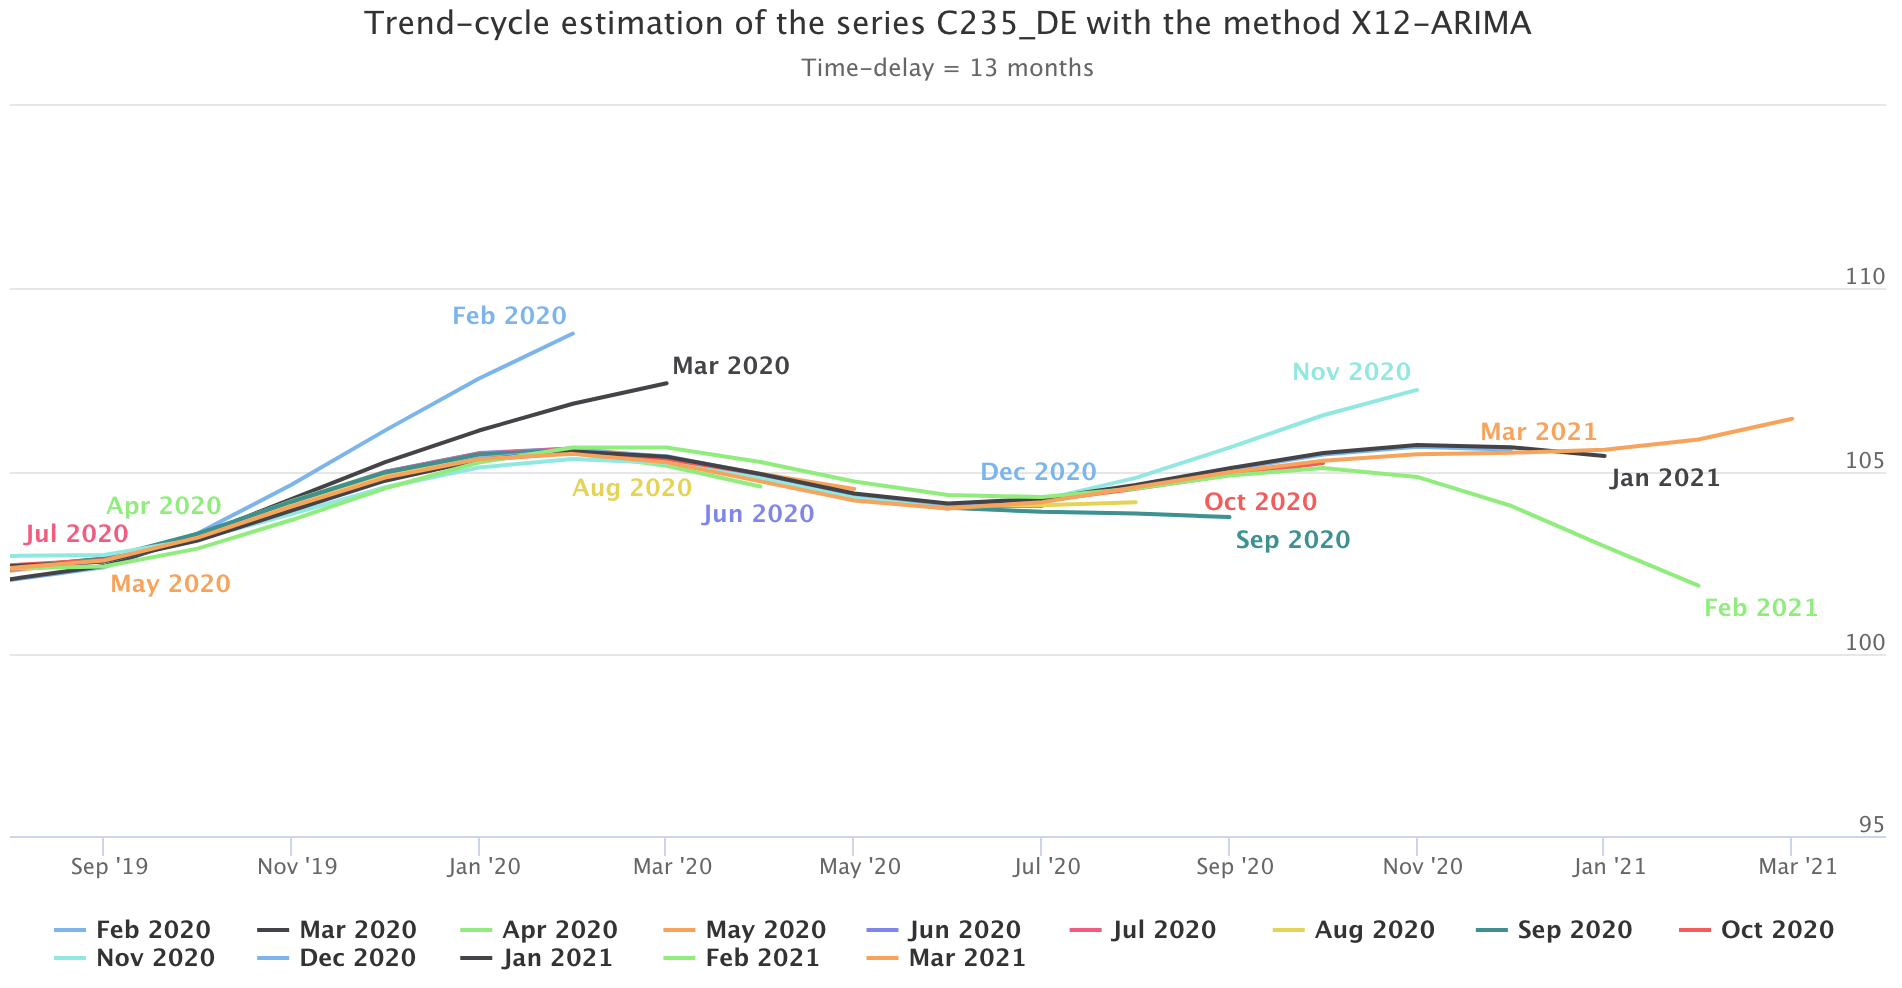
\includegraphics[width=0.95\textwidth]{img/C235DE_x13}
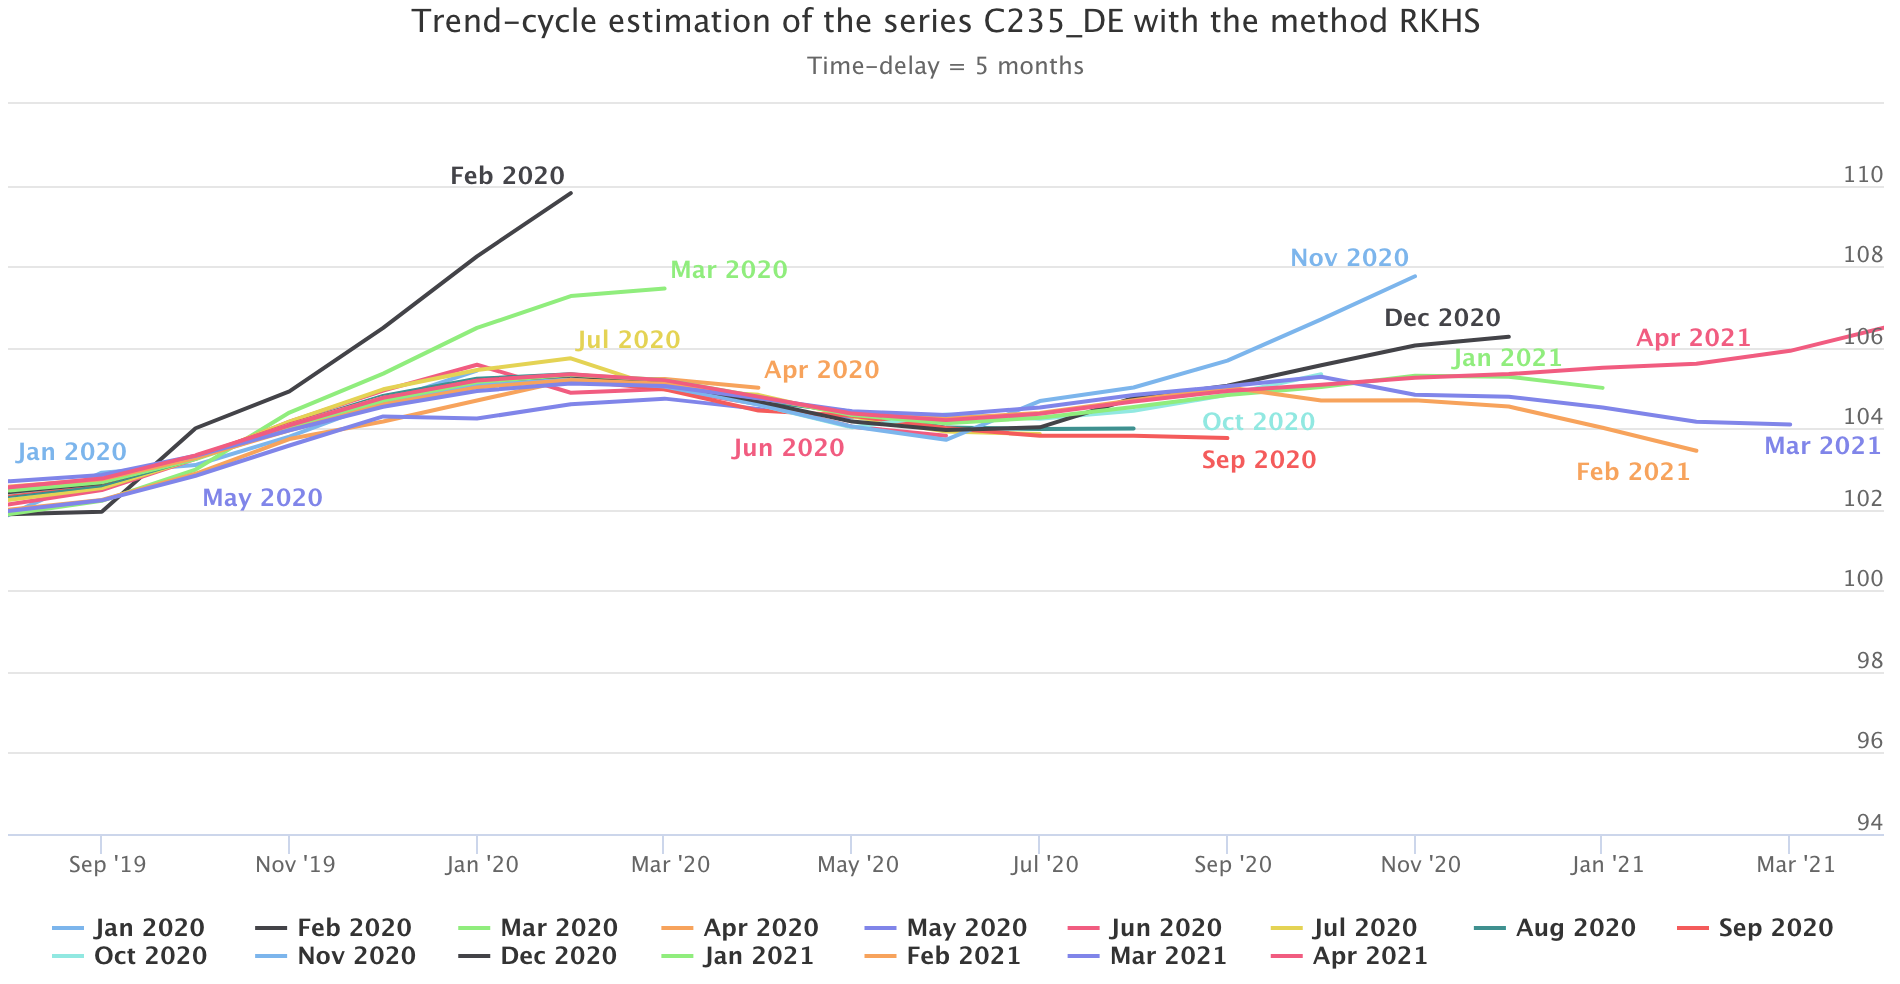
\includegraphics[width=0.95\textwidth]{img/C235DE_rkhs} 
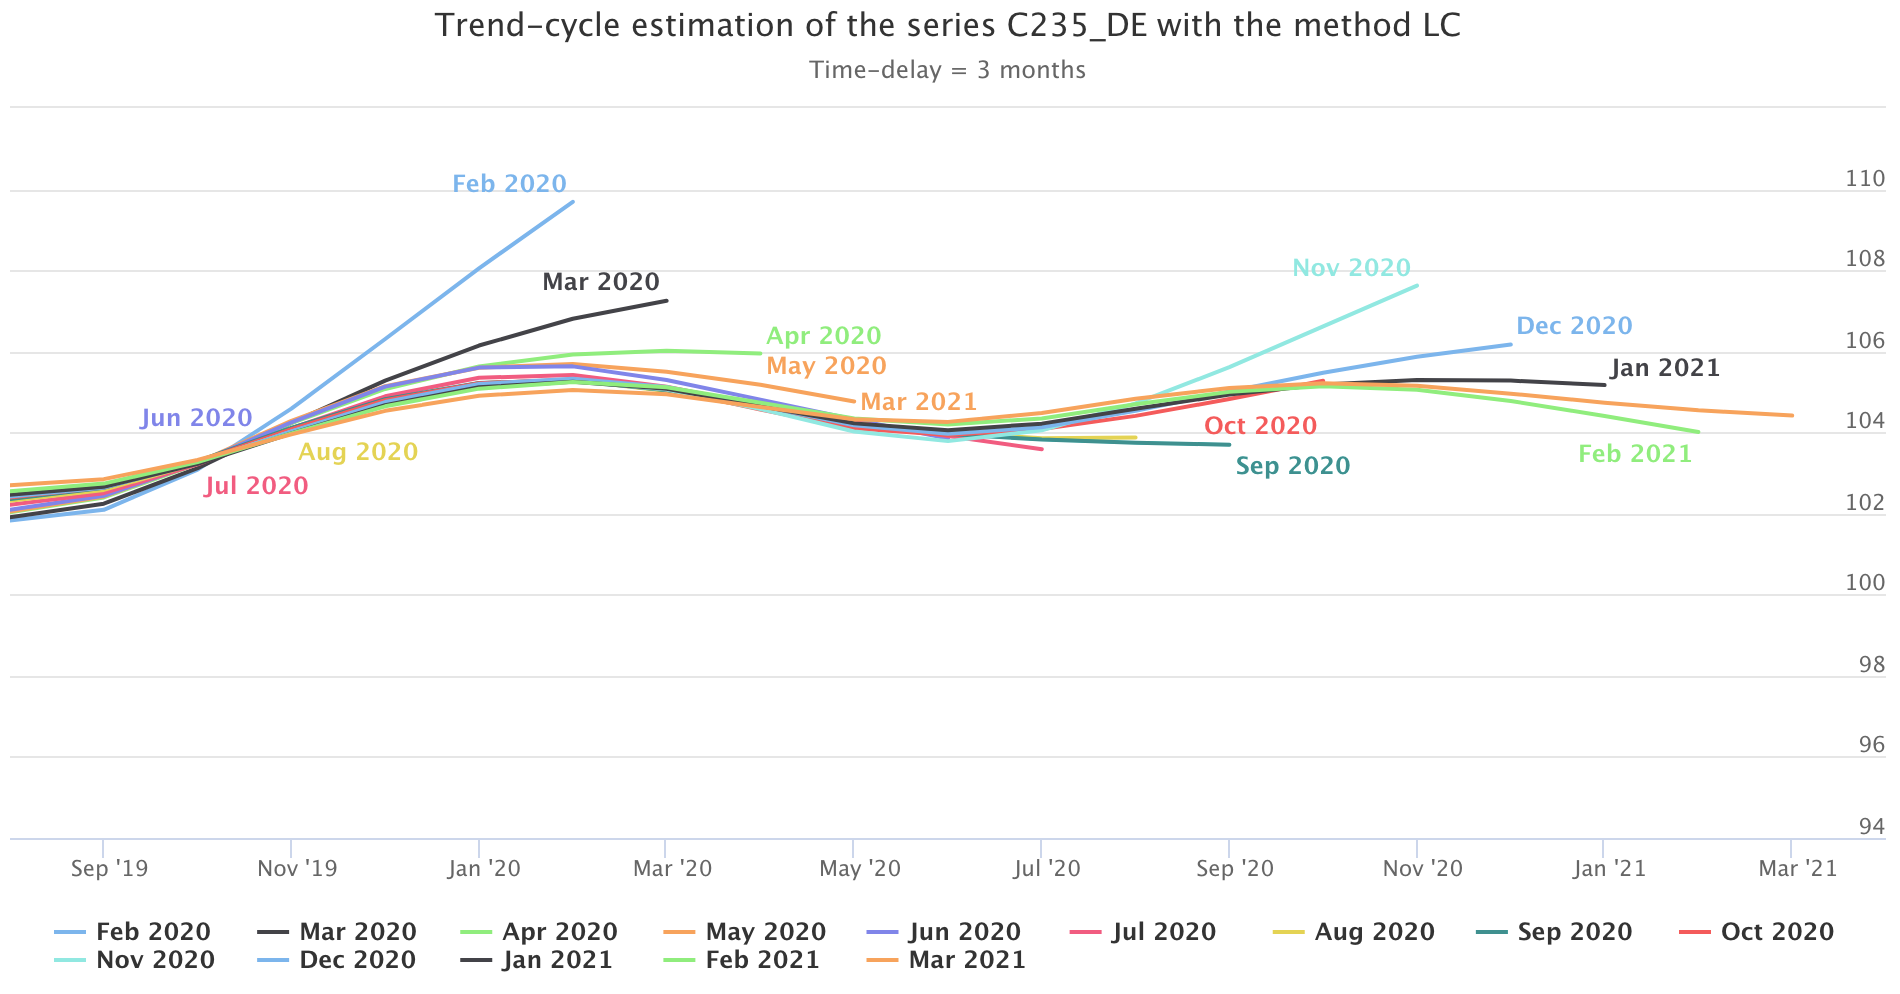
\includegraphics[width=0.95\textwidth]{img/C235DE_lc}
\caption{Estimates of the trend-cycle component for the industrial production index in the manufacture of cement, lime and plaster (C235) in Germany (turning point in February 2020).}
\label{fig:C235DEp1}
\end{figure*}

\begin{figure*}\centering
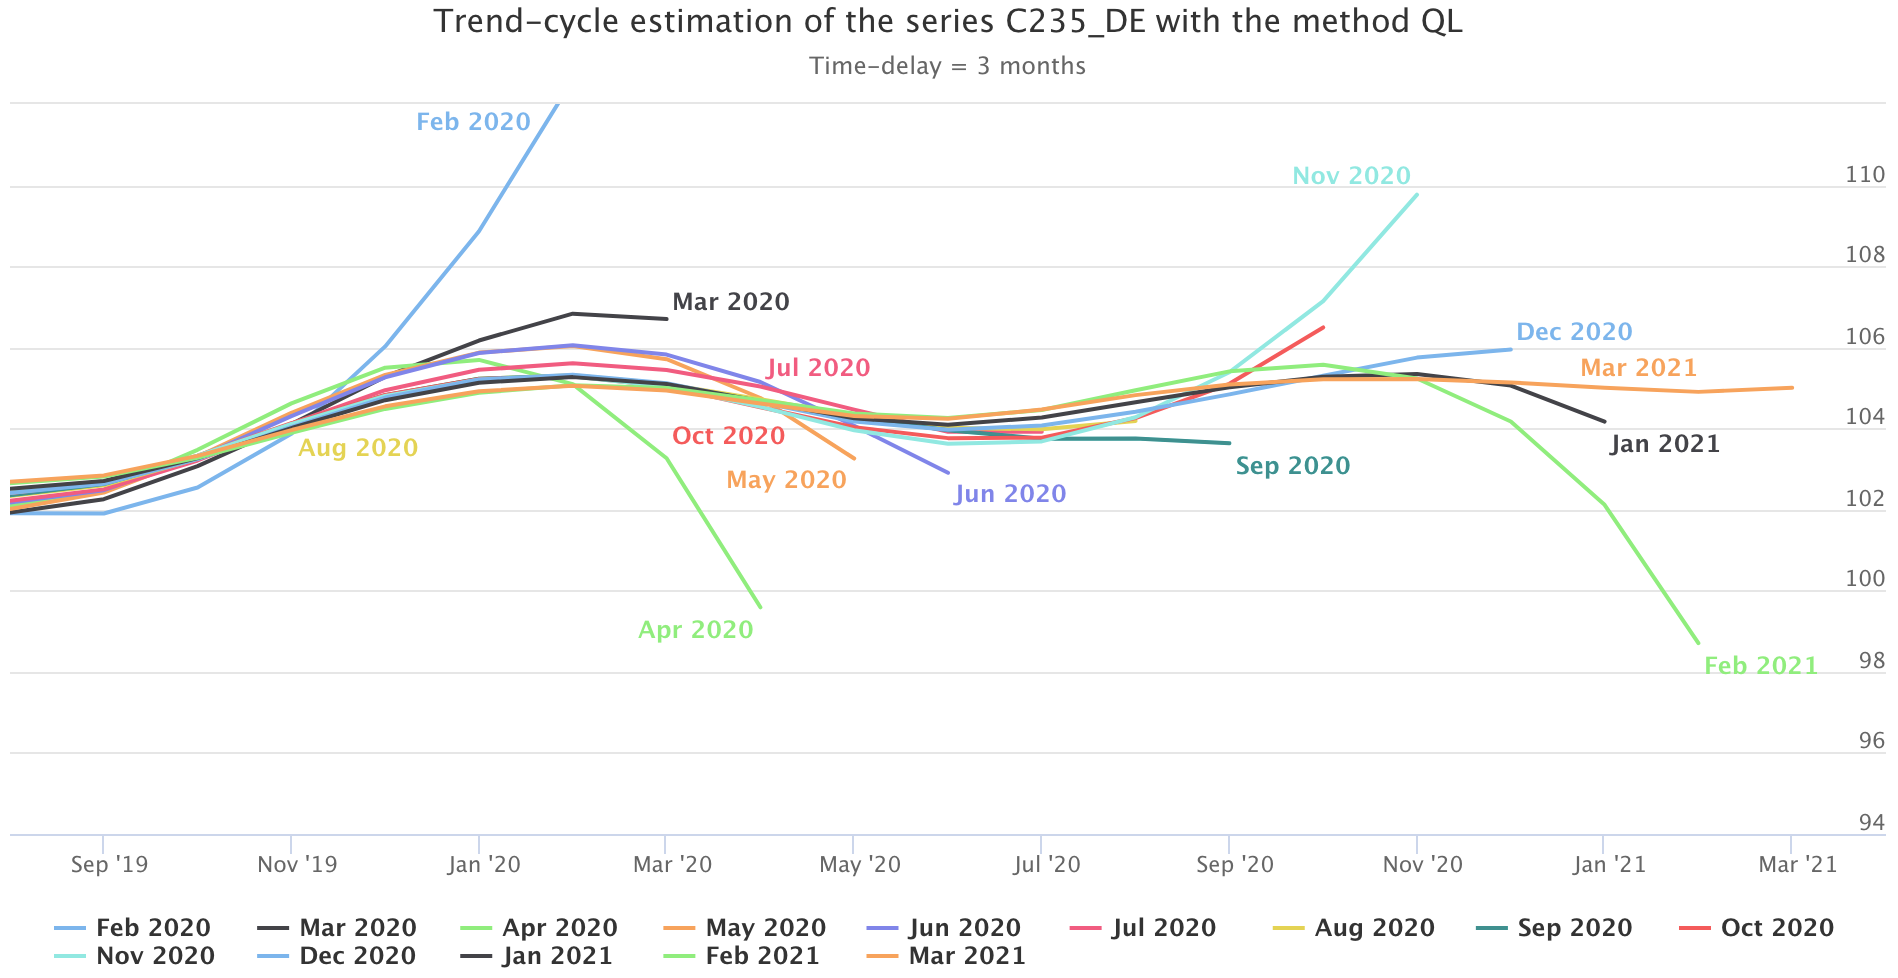
\includegraphics[width=0.95\textwidth]{img/C235DE_ql} 
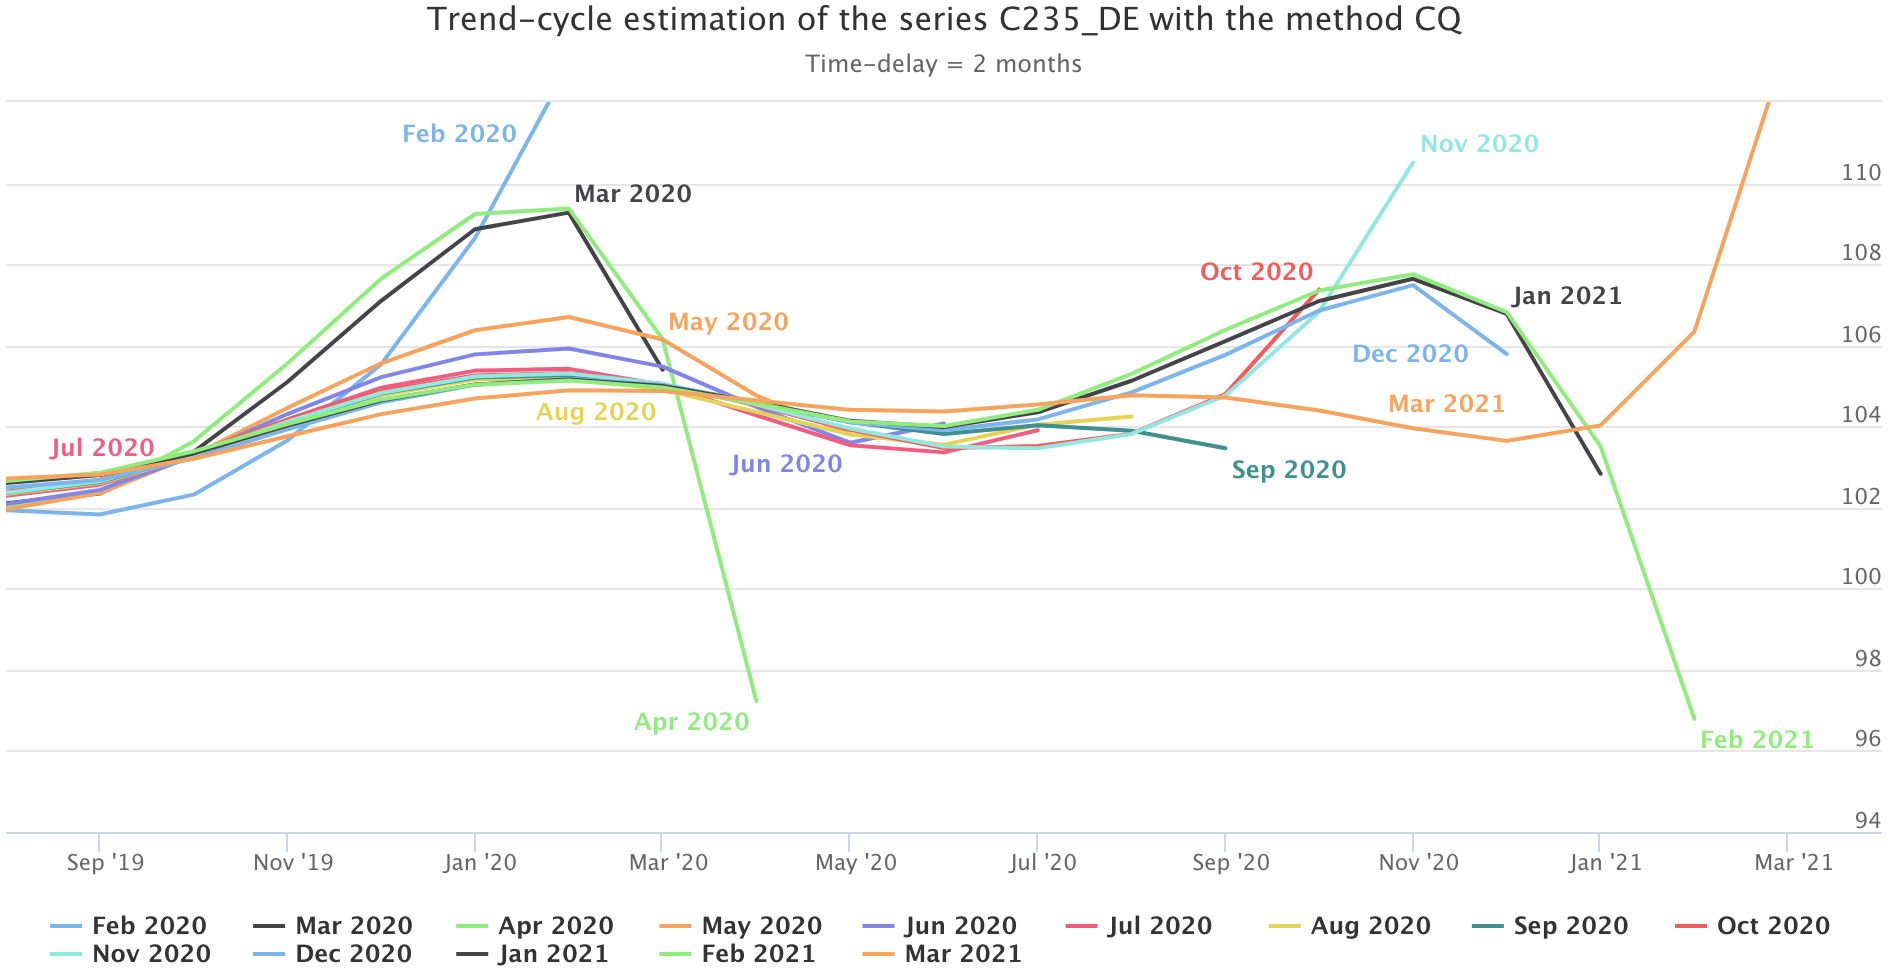
\includegraphics[width=0.95\textwidth]{img/C235DE_cq}
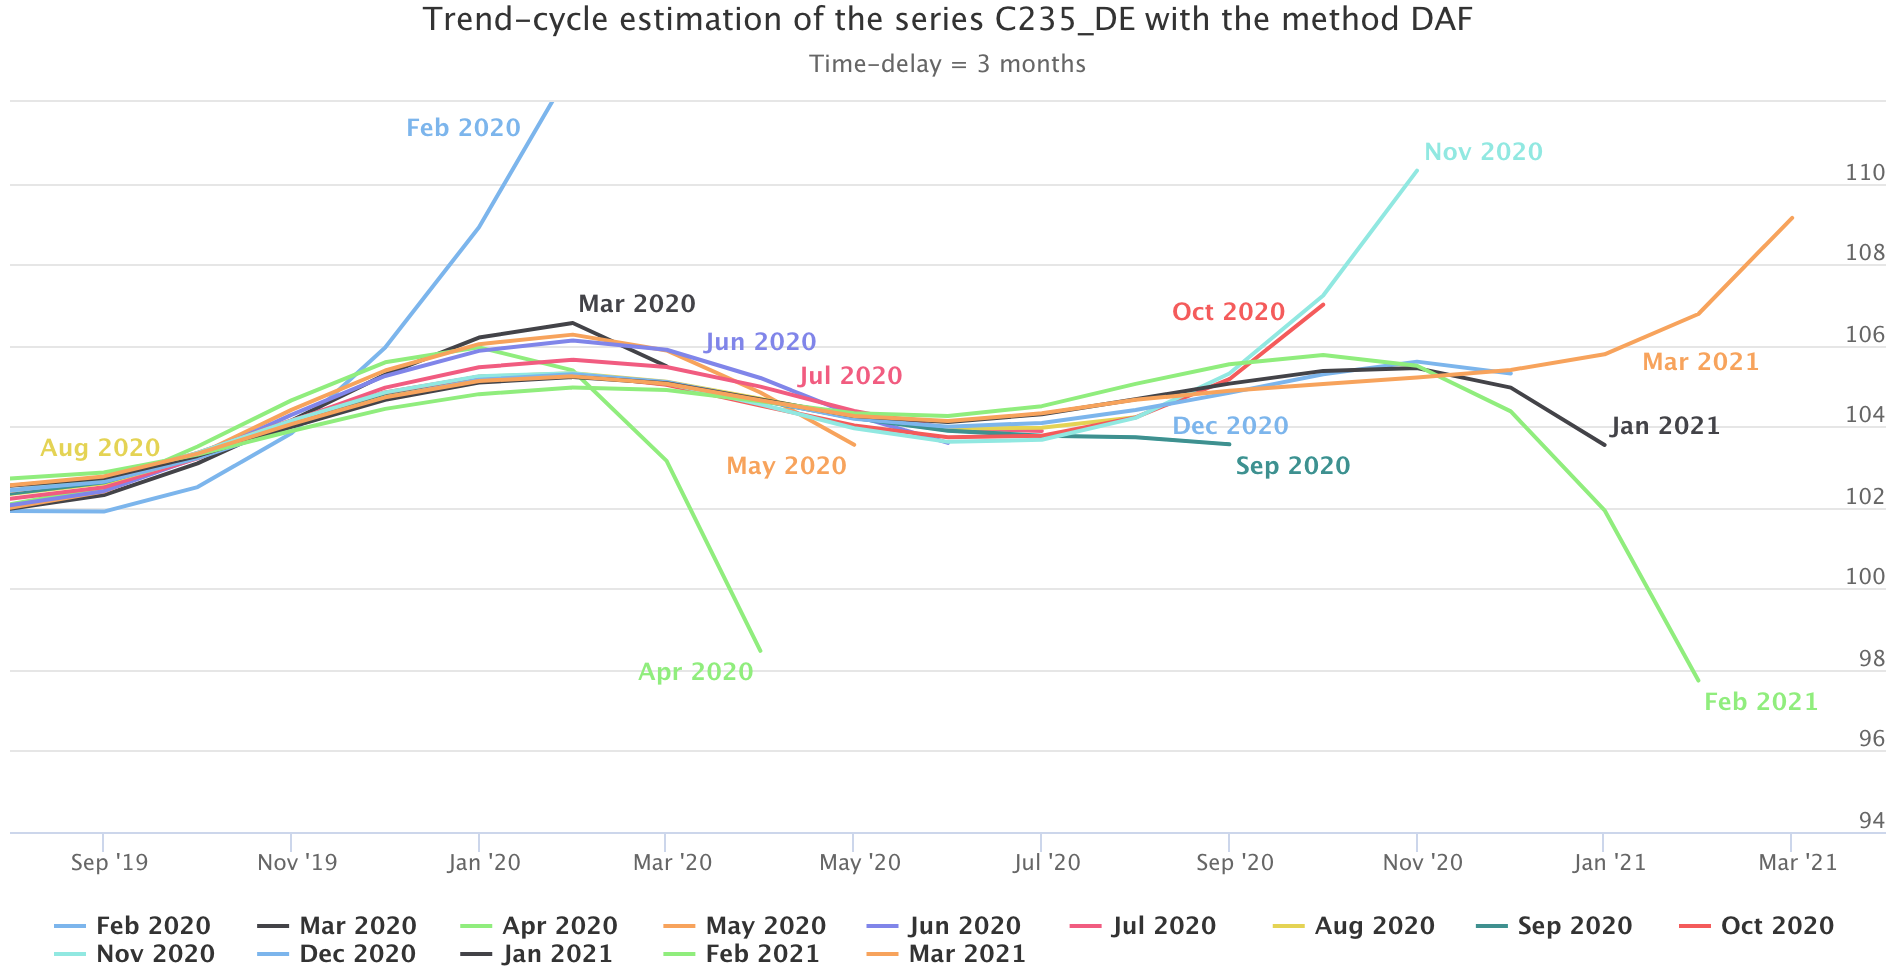
\includegraphics[width=0.9\textwidth]{img/C235DE_daf} 
\caption{Estimates of the trend-cycle component for the industrial production index in the manufacture of cement, lime and plaster (C235) in Germany (turning point in February 2020).}
\label{fig:C235DEp2}
\end{figure*}

\begin{figure*}\centering
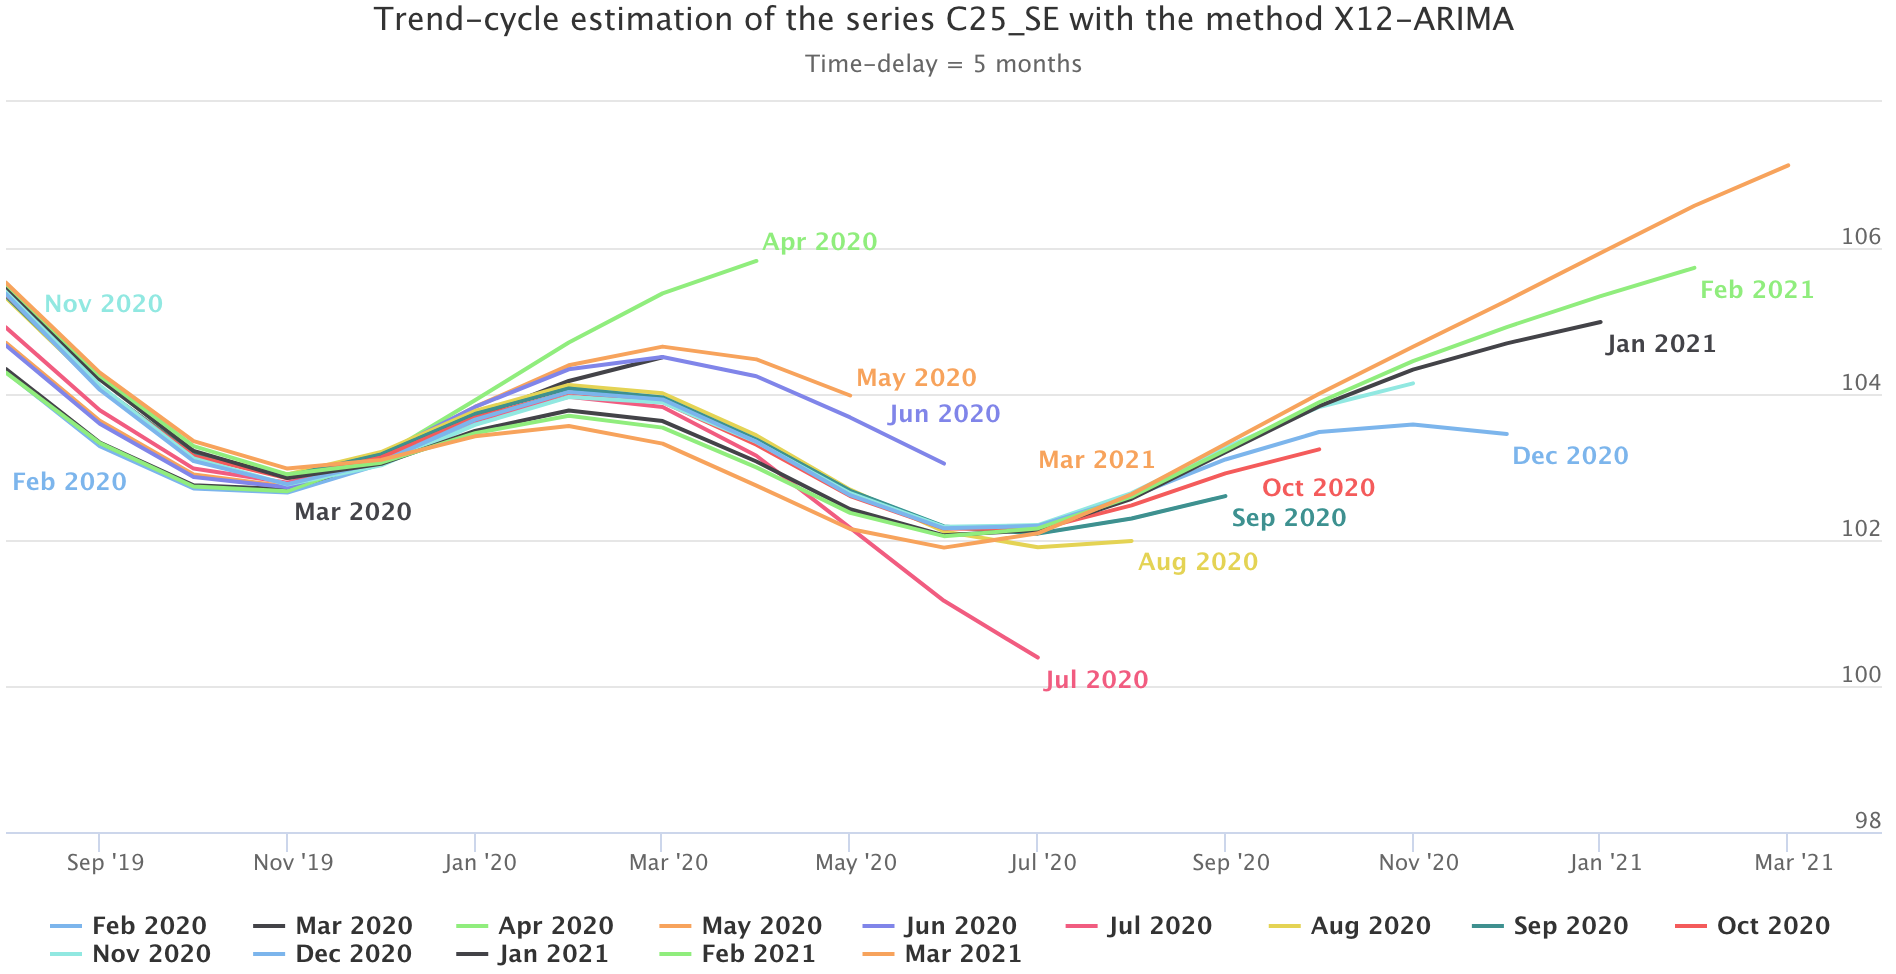
\includegraphics[width=0.9\textwidth]{img/C25SE_x13}
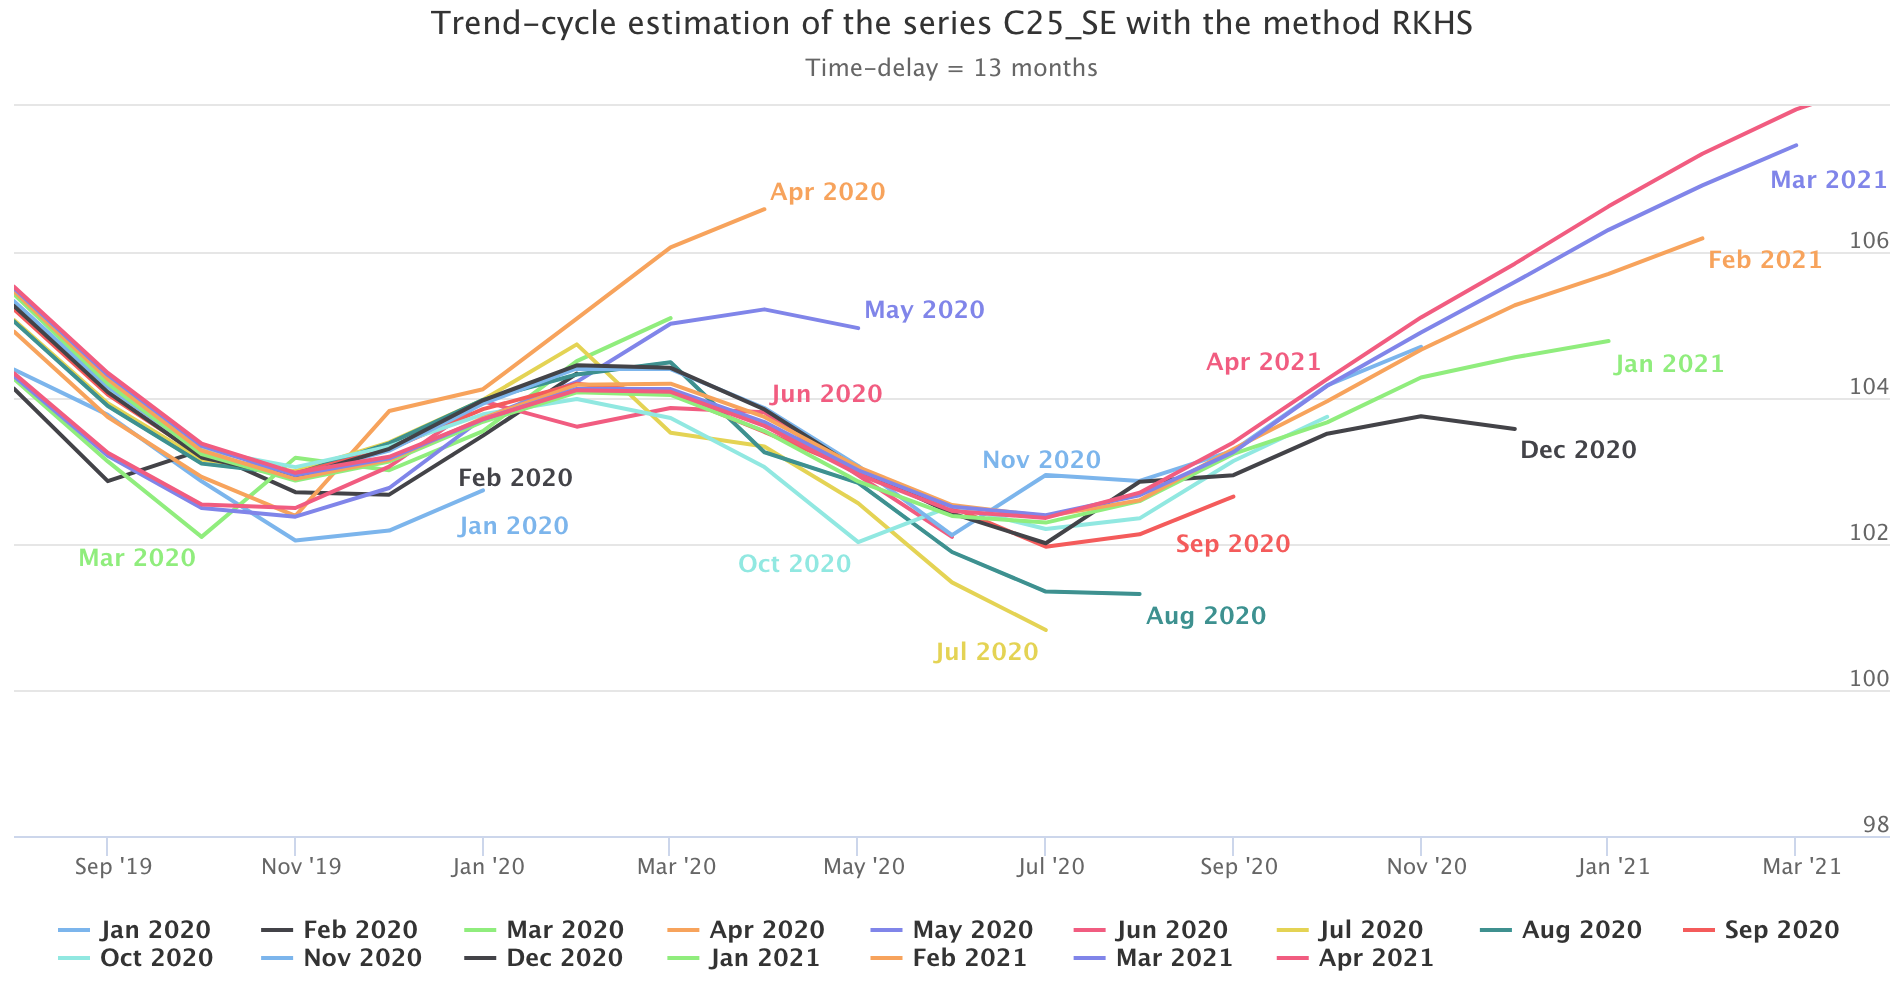
\includegraphics[width=0.9\textwidth]{img/C25SE_rkhs} 
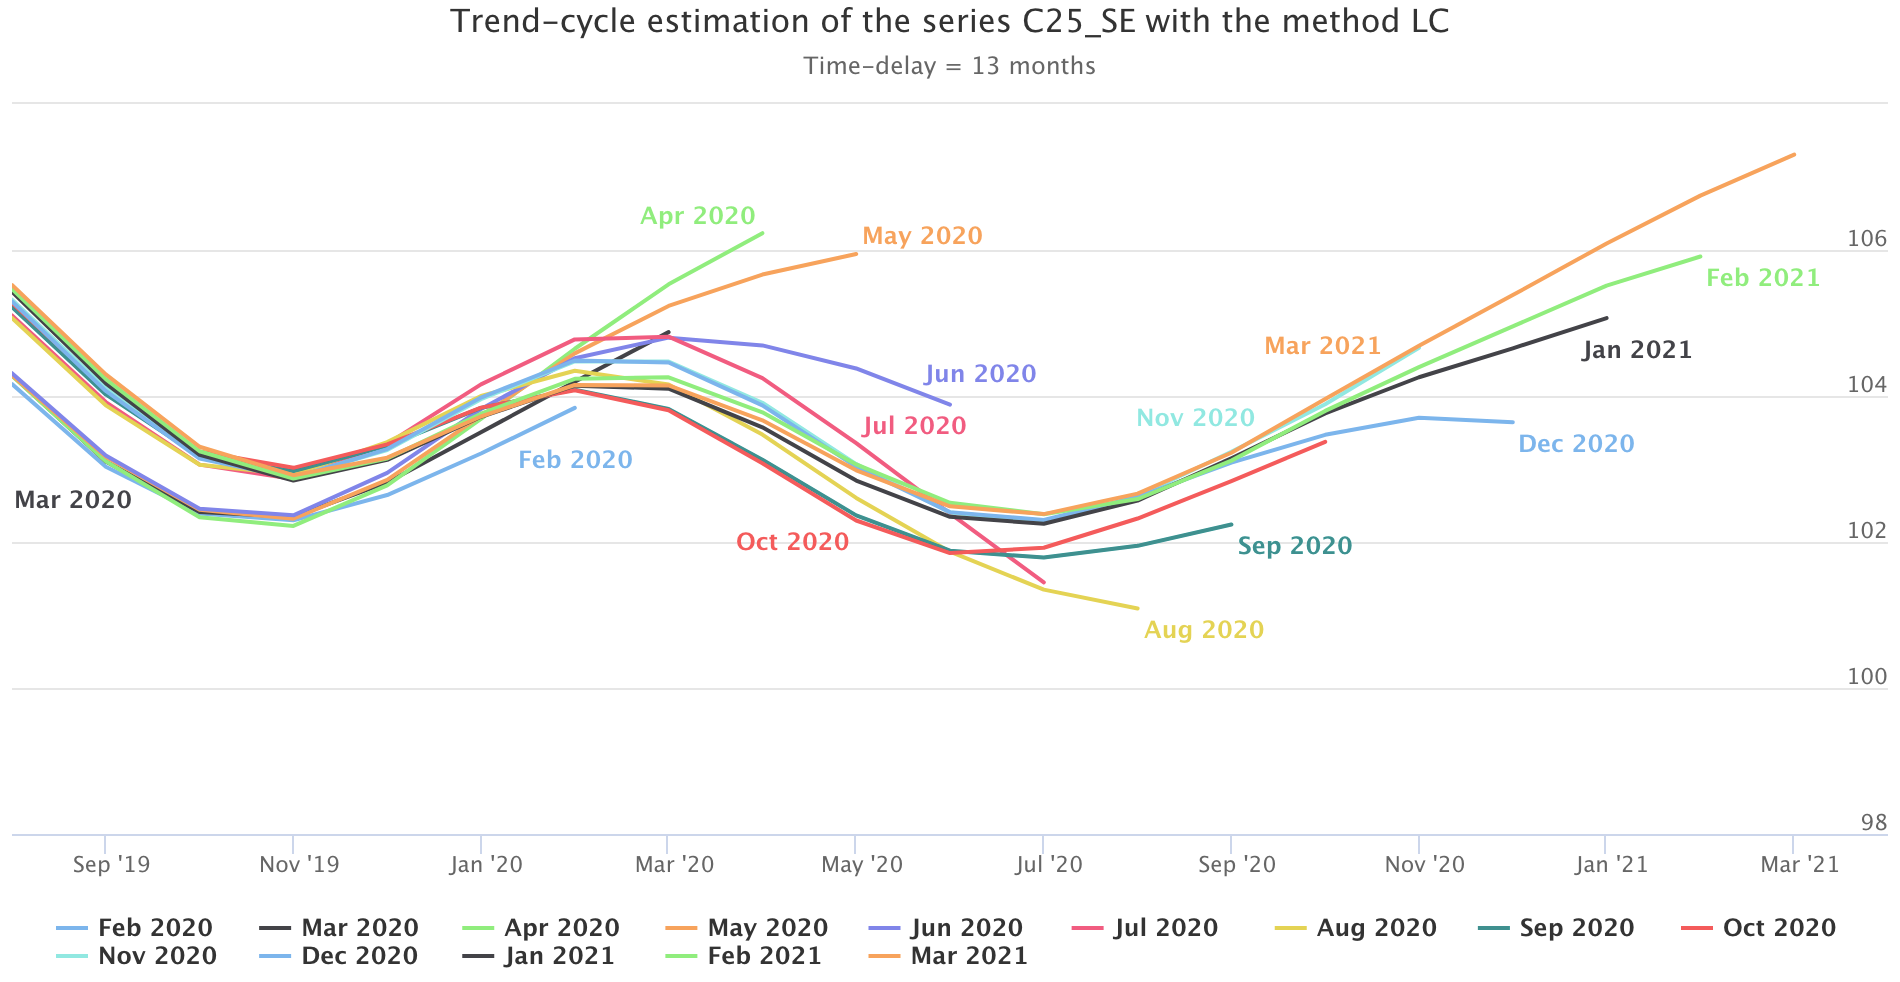
\includegraphics[width=0.9\textwidth]{img/C25SE_lc}
\caption{Estimates of the trend-cycle component for the industrial production index in the manufacture of fabricated metal products, except machinery and equipment (C25) in Sweden (turning point in February 2020).}
\label{fig:C25SEp1}
\end{figure*}

\begin{figure*}\centering
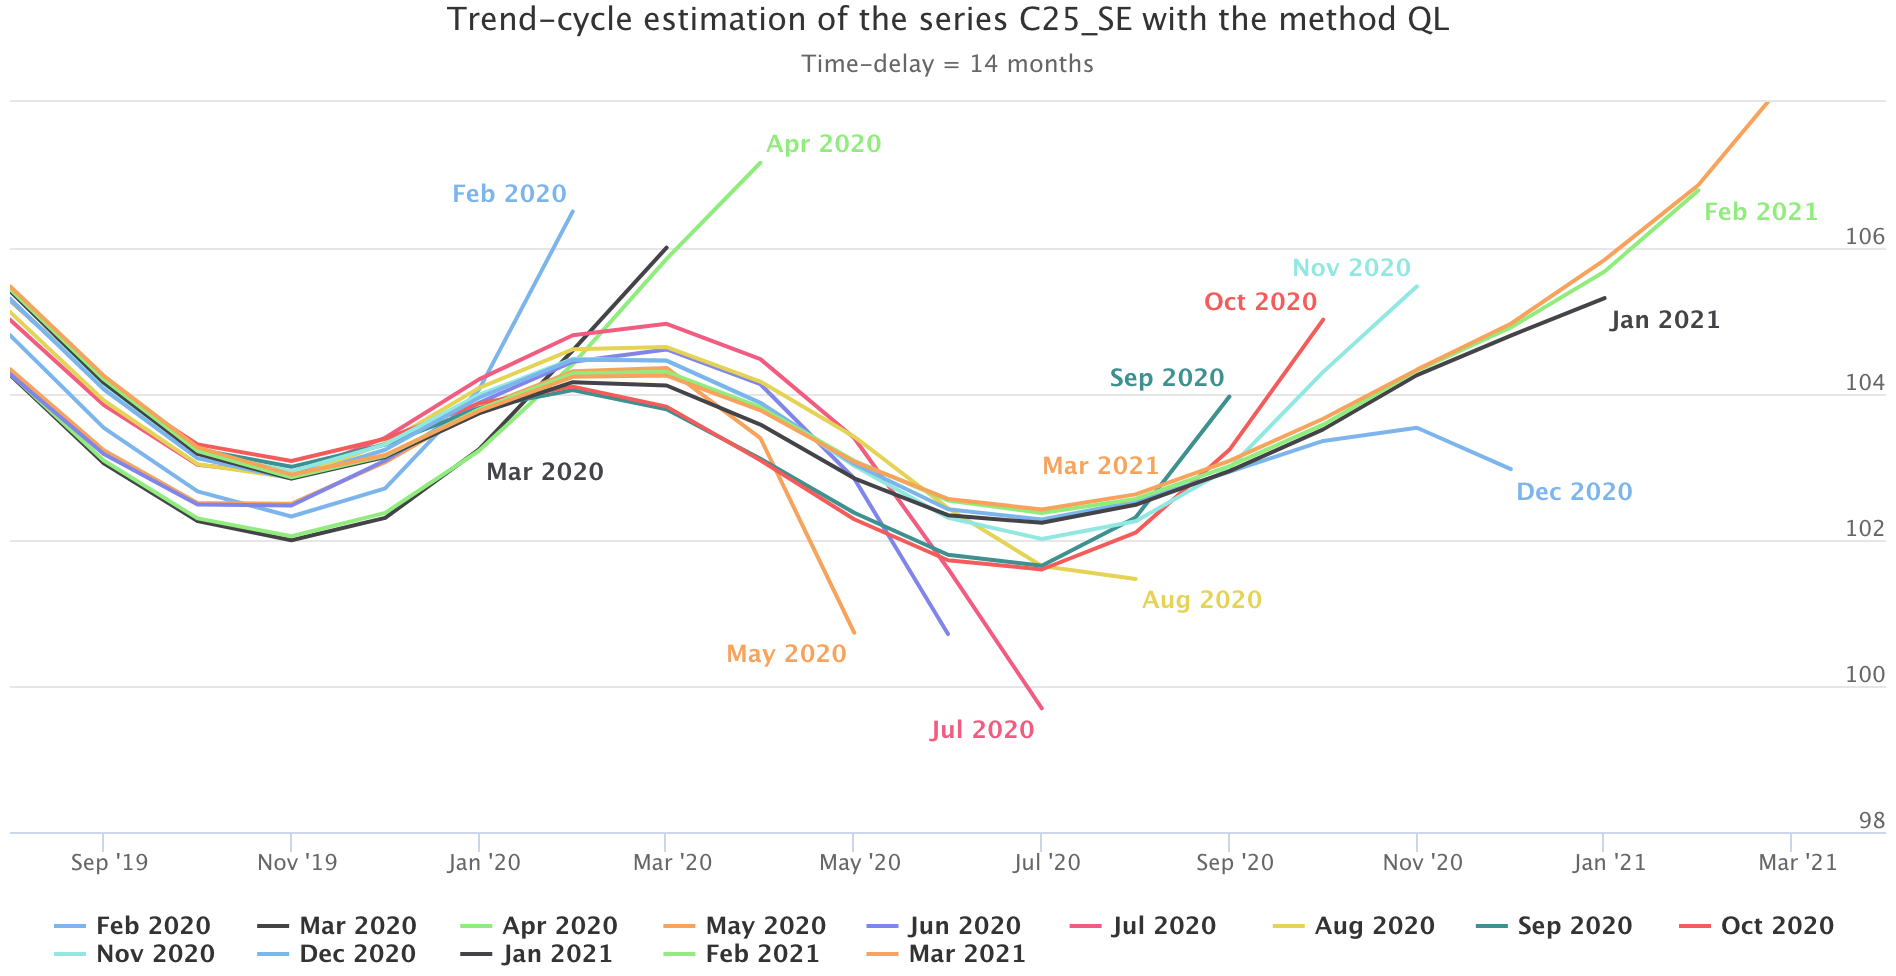
\includegraphics[width=0.9\textwidth]{img/C25SE_ql} 
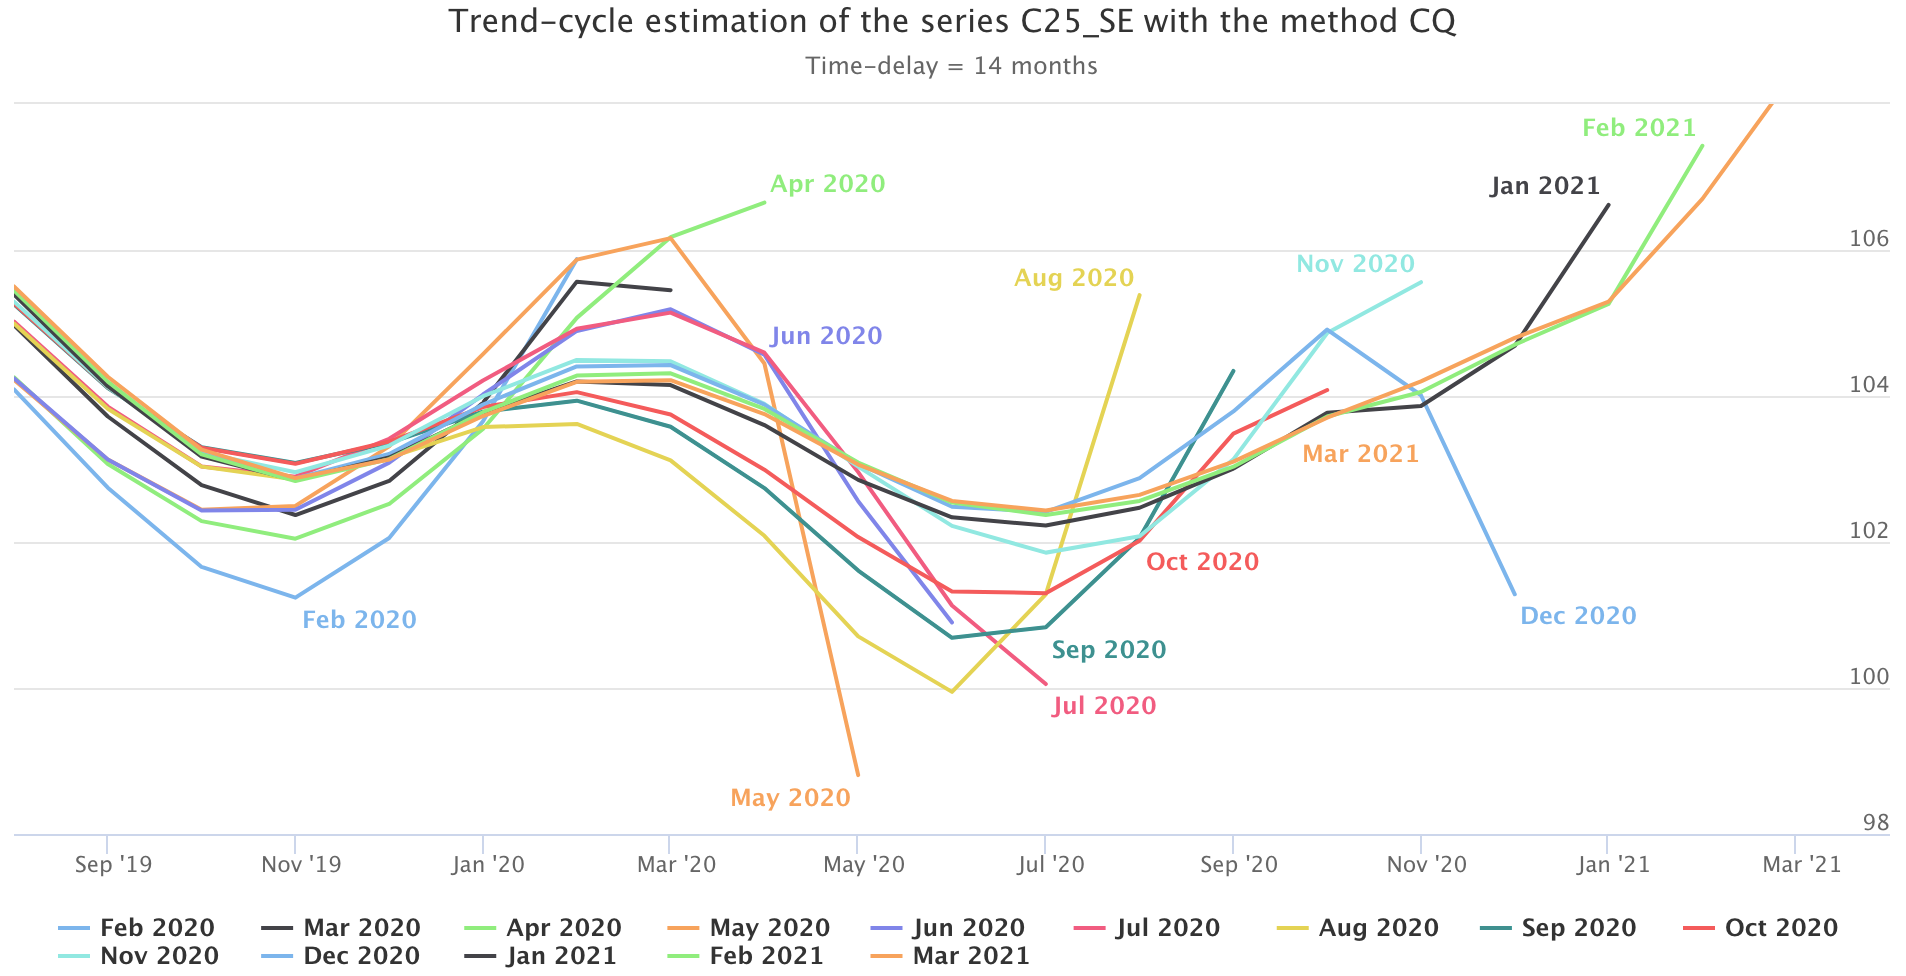
\includegraphics[width=0.9\textwidth]{img/C25SE_cq}
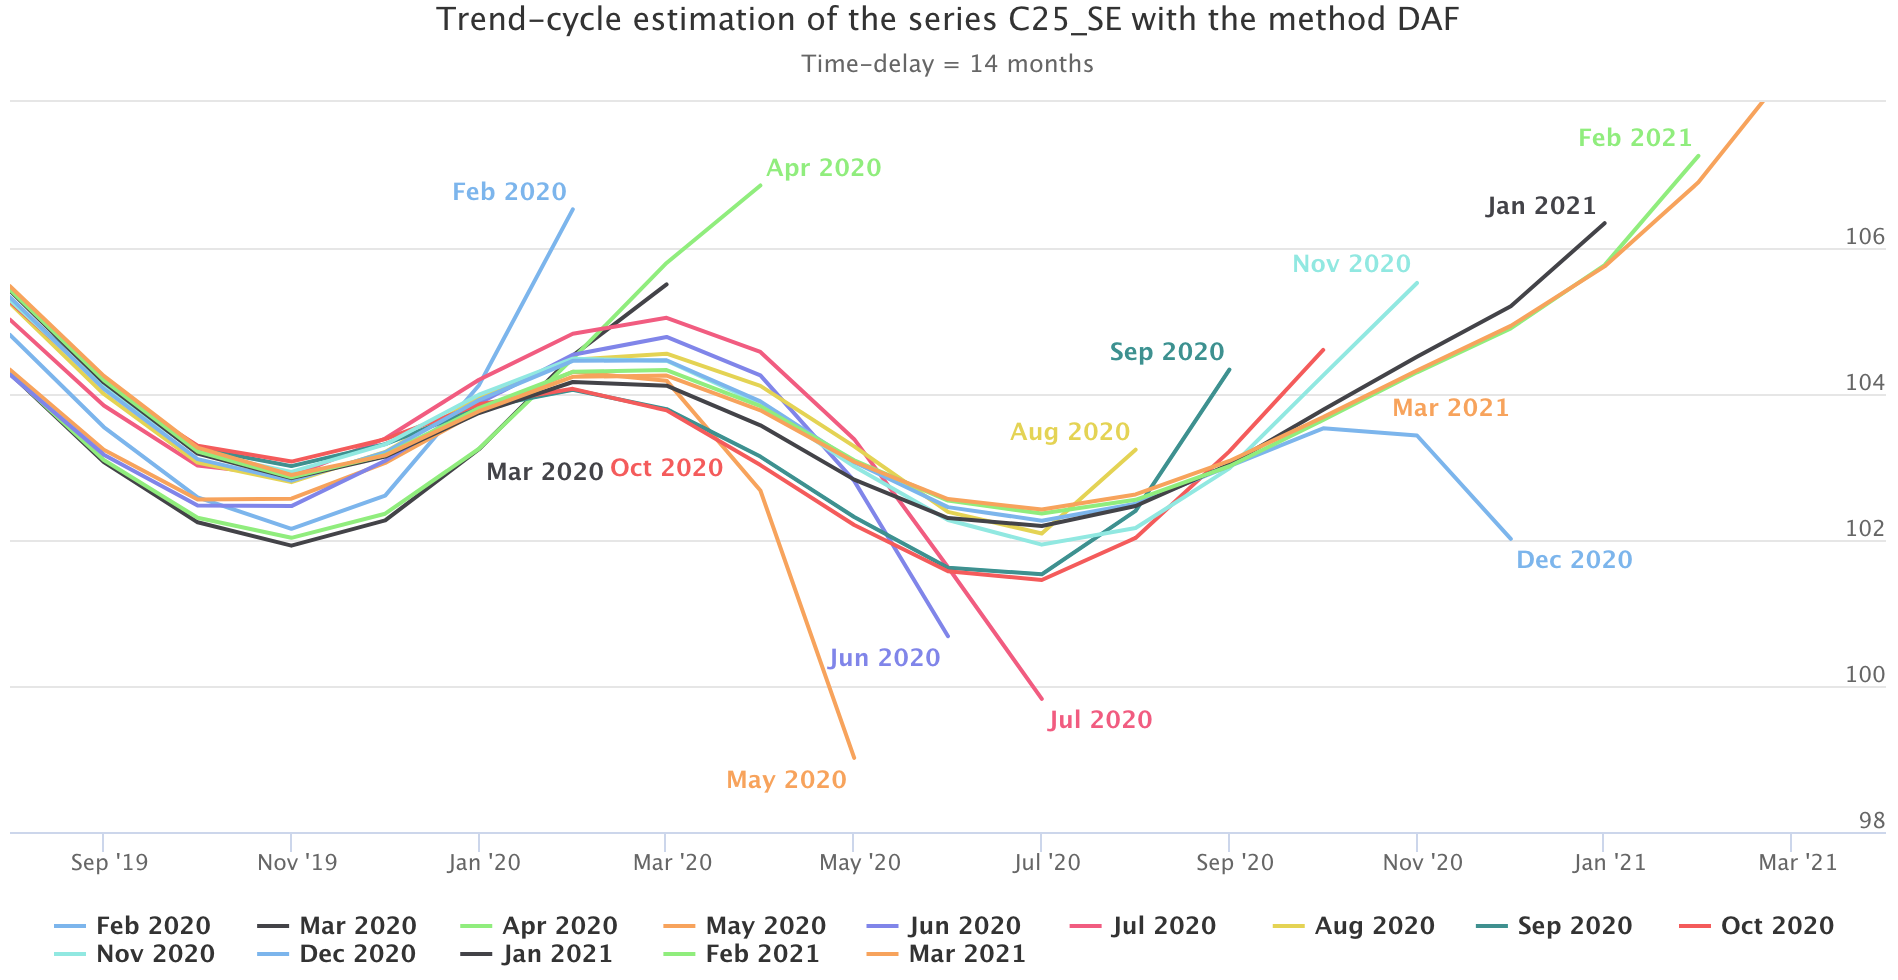
\includegraphics[width=0.9\textwidth]{img/C25SE_daf}
\caption{Estimates of the trend-cycle component for the industrial production index in the manufacture of fabricated metal products, except machinery and equipment (C25) in Sweden (turning point in February 2020).}
\label{fig:C25SEp2}
\end{figure*}

%----------------------------------------------------------------------------------------
%	REFERENCE LIST
%----------------------------------------------------------------------------------------

\bibliographystyle{chicago}
\makeatletter
% The filename has .bib extension that must be eliminated
\filename@parse{biblio.bib}
% parse stores the file name in base. Extension starts at the first dot, so don't use dots in file names.
\bibliography{\filename@base}
\makeatother


%----------------------------------------------------------------------------------------

\end{document}
